\documentclass[preprint,10pt,times]{elsarticle}

\usepackage{amssymb}
\usepackage{amsmath}
\usepackage{lineno}
\usepackage{geometry}
\geometry{letterpaper,top=4.3cm,bottom=4.3cm,left=4.8cm,right=4.8cm}
\usepackage{booktabs}
\usepackage{graphicx}
\usepackage{url}
\usepackage{setspace}
\doublespacing
\usepackage{enumitem}
\usepackage{hyperref}
\usepackage{orcidlink}

\journal{Pattern Recognition}

\begin{document}

\linenumbers

\begin{frontmatter}

\title{A Multi-Task Benchmark for Evaluating LLMs on Peer Review in Interdisciplinary Social Sciences}

\author[a]{Kai Qiao \orcidlink{0009-0000-0187-9190}}
\author[a,b]{Xiaoping Sheng\corref{cor1} \orcidlink{0000-0002-9310-6028}}
\ead{Shengxp68@126.com} % 紧跟在作者后面
\cortext[cor1]{Corresponding author.}
\author[a]{Zhenyu Li \orcidlink{0000-0002-6043-3479}}

\affiliation[a]{organization={School of Cultural Heritage and Information Management, Shanghai University},
              city={Shanghai},
              country={China}}

\affiliation[b]{organization={Research Academy of Cultural Heritage and Technology, Shanghai University},
              city={Shanghai},
              country={China}}

\begin{abstract}
As academic publishing continues to expand, peer review is facing increasing pressure. Large language models (LLMs) offer new possibilities for review assistance, Yet existing evaluations remain largely task-specific, with limited attention to multi-stage peer review processes, diverse evaluative perspectives, and cross-disciplinary settings. We construct a multi-task benchmark for interdisciplinary social sciences using open peer-review data from PeerJ, Nature, PLOS, and ICLR, spanning fields such as social science, data science, and psychology. The benchmark comprises 2,769 papers, 7,432 review reports, and 24,632 review--response dialogue pairs. We design three progressive tasks to evaluate LLM performance in review dimension coverage, reply resolution judgment, and round-level acceptability judgment, thereby providing a more process-aware benchmark framework. Experiments on six frontier LLMs show that the models can reasonably reproduce human reviewers' attention to core dimensions such as methodological rigour in the coverage task. However, their performance degrades markedly when judging whether reviewer concerns are reflected as resolved in author responses and when making round-level acceptability judgments, revealing clear limitations in higher-order evaluative reasoning and judgment calibration. Different models also exhibit stable, distinctive biases: some overemphasise impact or judge concerns as resolved too optimistically, while others tend toward more negative assessments. These findings indicate that single-task frameworks may overestimate broader peer-review capabilities and that deploying these models without task-specific calibration may introduce systematic, model-dependent biases. The proposed benchmark offers a more comprehensive multi-task framework for the standardized evaluation of LLMs in open peer review.
\end{abstract}

\begin{highlights}
\item Proposed a multi-task benchmark for evaluating LLMs in peer review.
\item Built a large-scale dataset for interdisciplinary social science peer review.
\item LLMs show human-like attention patterns in review coverage.
\item LLMs remain limited in rebuttal assessment and acceptance prediction.
\item Single-task evaluation is insufficient for assessing LLMs in peer review.
\end{highlights}

\begin{keyword}
Peer review \sep Large language models \sep Evaluation benchmark \sep Interdisciplinary social sciences \sep Multi-task evaluation
\end{keyword}

\end{frontmatter}

%%======================================================================
\section{Introduction}
\label{sec:intro}
%%======================================================================

In recent years, the rapid advancement of large language models (LLMs) has profoundly transformed the field of AI, achieving breakthrough performance in natural language processing, reasoning, and generative tasks. Leading models such as ChatGPT, Claude, Grok, and Gemini have significantly advanced the state of the art, demonstrating strong performance across text understanding, reasoning, and content generation~\cite{ref1}. These capabilities have been progressively extended into scientific research, fundamentally transforming traditional research paradigms and accelerating the advancement of scientific disciplines. In particular, LLMs have evolved from conventional text-generation tools into autonomous agents capable of supporting scientific inquiry, including literature review, hypothesis generation, experimental design, data analysis, and result interpretation~\cite{ref2}. A comprehensive survey of LLMs across more than 260 scientific fields reviewed datasets, evaluation tasks, and model characteristics across diverse domains and modalities, highlighting their substantial potential for scientific research.~\cite{ref3}. The evolution of LLMs has reshaped their role in scientific research and redefined how humans collaborate with AI in this process.~\cite{ref4}. This trend has also extended to key stages of academic publishing, particularly peer review.

Peer review is the cornerstone of academic publishing and the primary mechanism for safeguarding research quality. However, the rapid growth of global research output and the increasing complexity of interdisciplinary scholarship have posed major challenges to traditional peer review systems. This has sparked growing interest in integrating AI into the review process~\cite{ref5}. With strong text understanding and generation capabilities, LLMs are well suited to supporting review related tasks. Recent surveys on automated scholarly paper review highlight their transformative potential, while also noting persistent challenges such as limited review depth, over-positivity, and hallucination.~\cite{ref6}. As these models continue to improve, developing robust benchmark frameworks with well-constructed datasets and comprehensive evaluation protocols becomes essential for tracking progress and aligning model capabilities with the practical demands of peer review.

In prior work, Kang et al.\ (2018) introduced PeerRead, the first large-scale peer review dataset, comprising 14.7K paper drafts and 10.7K expert reviews from ACL, NeurIPS, and ICLR, which has since served as a foundational resource for subsequent research~\cite{ref7}. Building on this, Li et al.\ (2025) constructed a large-scale benchmark of 1,683 papers and 6,495 expert reviews from ICLR and NeurIPS, and employed five LLMs to generate reviews for comparison with human counterparts. Using semantic similarity analysis and structured knowledge graph metrics, they found that LLMs perform well on descriptive content but exhibit notable deficiencies in critical reasoning~\cite{ref8}. REMOR introduces explicit reasoning and multi-objective reinforcement learning to improve LLM performance in peer review, with experiments on PeerRT evaluating review quality and manuscript relevance~\cite{ref9}. MMReview provides a multidisciplinary and multimodal benchmark for LLM based peer review evaluation, covering 17 research domains and 13 tasks, including stepwise review generation, outcome prediction, and adversarial robustness. However, its evaluation still focuses primarily on review generation and decision related tasks, without explicitly assessing whether models can judge the adequacy of author rebuttals~\cite{ref10}.

Despite these advances, notable gaps remain. Most existing benchmarks cover only a few disciplines, leaving model generalizability largely untested. Current work also centres on reviewer-side tasks, paying limited attention to other important aspects of peer review, such as author rebuttals, which remain relatively underexplored. Moreover, existing benchmarks tend to break peer review into fine-grained, isolated subtasks. While this approach has diagnostic value, when LLMs have yet to be integrated into peer review practice, a unified framework evaluating model performance across broader tasks may be more valuable than increasingly narrow task decomposition. Addressing these gaps is essential for advancing the real-world application of LLMs in scholarly evaluation. To this end, this study first constructs a new dataset from open peer review data across interdisciplinary fields related to the social sciences. We then propose a benchmark framework covering three core tasks: review dimension coverage, reply resolution judgment, and round-level acceptability judgment. Finally, we systematically evaluate six state-of-the-art LLMs across these tasks to examine cross-model differences and identify their strengths and limitations in peer-review settings.

%%======================================================================
\section{Related Work}
\label{sec:related}
%%======================================================================

\subsection{LLMs for Scientific Tasks}
\label{sec:llms-sci}

The capabilities of LLMs are primarily determined by parameter scale, architecture, and training strategy. Beyond a certain size threshold, emergent abilities such as complex reasoning, instruction-following, and few-shot learning arise that smaller models lack~\cite{ref11}. Peer review requires simultaneous comprehension of lengthy academic texts, multidimensional critique generation, assessment of argumentative rigour, and integrative decision-making, placing stringent demands on deep language understanding and reasoning. As academic papers also contain multimodal content (figures, equations, visualisations), models with mixed text-image processing capabilities hold an inherent advantage. Smaller open-source models (e.g., 7B--13B) often fall short of these demands and require extensive fine-tuning~\cite{ref12,ref13}. This study, therefore, focuses on frontier models to establish a more informative capability benchmark.

GPT-4 is OpenAI's multimodal model that supports text and image inputs and consistently leads benchmarks such as MMLU and HumanEval~\cite{ref14}. GPT-4o is its efficiency-optimised variant, maintaining comparable reasoning performance at substantially lower latency and cost~\cite{ref15}. Claude Opus and Claude Sonnet, developed by Anthropic, represent the highest-capability and balanced-efficiency tiers, respectively~\cite{ref16}. Notably, the Claude series exhibits a conservative, consistent judgment style that may benefit peer-review scenarios that require precise rather than sycophantic assessment. DeepSeek R1 employs a Mixture-of-Experts architecture with reinforcement learning-enhanced reasoning. Gao et al.\ (2025) found its classification accuracy second only to Claude, though with notably slower inference~\cite{ref17}. Gemini 3 Pro, by Google DeepMind, natively supports text, image, audio, and video processing and maintains frontier performance on graduate-level reasoning benchmarks such as GPQA Diamond~\cite{ref18}. The Grok series by xAI has also demonstrated competitive performance~\cite{ref19}, but was excluded due to limited access during the study period.

In total, six models---GPT-4, GPT-4o, Claude Opus 4.6, Claude Sonnet 4.6, DeepSeek R1, and Gemini 3 Pro---were selected, spanning four providers and encompassing dense Transformer, MoE, and natively multimodal architectures. All consistently rank within the frontier tier on independent leaderboards such as Chatbot Arena~\cite{ref20} and Artificial Analysis, enabling meaningful cross-paradigm comparisons on peer-review tasks.

\subsection{Taxonomy of Peer Review Comments}
\label{sec:taxonomy}

A central challenge in AI-assisted peer review research is determining how best to evaluate the quality of AI-generated review comments. While computational semantic similarity has been used to measure alignment between AI and human reviews~\cite{ref21}, this method falls short. Peer review is not simply a summary of a manuscript but a complex critical analysis that involves methodological rigour, novelty, literature positioning, and the quality of exposition. Thus, the main argument is that establishing a dimensional taxonomy for review comments enables a more principled assessment of LLM reviewing capabilities at the cognitive level.

To address the need for clearer classification, several frameworks analyse review comments. Ortega (2022) grouped PubPeer comments into seven severity levels, showing diverse peer review perspectives~\cite{ref22}. Sizo et al.\ (2025) identified six categories that describe review quality at a macro level~\cite{ref23}. In terms of annotated dataset construction, Ghosal et al.\ (2022) built a multi-layered scheme from 1,199 ICLR 2018 reviews as a reference~\cite{ref24}. A growing consensus has emerged regarding specific dimensional frameworks. Yuan et al.\ (2022) proposed a popular taxonomy: Clarity, Soundness \& Correctness, Originality, and similar aspects~\cite{ref25}. Shin et al.\ (2025) used GPT-4o to identify aspects without supervision, further confirming this framework's robustness~\cite{ref26}. Wu et al.\ (2022) treated review--reply pairs as arguments~\cite{ref27}, while Kennard et al.\ (2022) marked the structure of review discussions~\cite{ref28}. These studies help researchers explore reply resolution and response evaluation.

Despite these advances, no single standard exists for classifying review comments. In addition, priorities differ across fields---experimental sciences value reproducibility, while social sciences emphasise the appropriate theoretical frameworks.

\subsection{Benchmarking LLMs for Peer Review}
\label{sec:benchmarking}

Leveraging LLMs to assist or automate peer review has emerged as a prominent research direction in recent years, accompanied by rapid progress in benchmark construction. Benchmarks are essential for assessing the practical capabilities of novel technologies~\cite{ref29}. Zhuang et al.\ (2025) provided a systematic survey of automated scholarly reviewing in the LLMs era, identifying both the transformative potential and persistent challenges of LLMs in this domain, including limited review depth, positivity bias, and hallucination~\cite{ref6}.

At the dataset level, Kang et al.\ (2018) introduced PeerRead, the first large-scale peer review dataset comprising 14,700 papers and 10,700 expert reviews from ACL, NeurIPS, and ICLR, laying the groundwork for subsequent research~\cite{ref7}. Since then, datasets have expanded considerably in both scale and disciplinary coverage. Lin et al.\ (2023) constructed MOPRD, a multidisciplinary dataset spanning biology, computer science, and environmental science, capturing the full review workflow---including multiple manuscript versions, review reports, meta-reviews, author rebuttals, and editorial decisions~\cite{ref30}. Dycke et al.\ (2023) further broadened the scope with NLPeer, incorporating data from multidisciplinary journals such as PLOS and eLife, with particular attention to ethical data acquisition. Their systematic survey of 53 existing datasets revealed that 37 originated from ML/NLP conferences hosted on OpenReview, while social science domains remained virtually unrepresented~\cite{ref31}.

At the benchmark framework level, existing studies have gradually moved beyond single-task feasibility tests toward broader evaluations of LLMs in scholarly peer review. Early work mainly examined isolated review-related abilities. Liu and Shah (2023), for example, evaluated GPT-4 on error detection and checklist verification, showing that LLMs can support reviewers but remain insufficient for independent, end-to-end reviewing~\cite{ref32}. Subsequent studies expanded the scope of evaluation from isolated assistance tasks to more structured benchmark settings. AAAR-1.0 introduced expert-level tasks such as equation inference, experiment design, weakness identification, and review quality assessment~\cite{ref33}, while Li et al.\ (2025) compared LLM-generated and human reviews through semantic similarity and knowledge graph metrics, showing that LLMs perform relatively well in descriptive content but remain limited in critical reasoning~\cite{ref8}. Recent work has further broadened benchmark design in terms of scale, modality, and review quality dimensions. MMReview spans 17 disciplines and 13 evaluation tasks~\cite{ref10}. ReviewEval incorporates retrieval-augmented factual verification to assess AI-generated review quality~\cite{ref21}, and ReviewAgents explores multi-agent collaboration to improve the comprehensiveness and reliability of generated reviews~\cite{ref34}. Zhou et al.\ (2024) further demonstrated that fluent review generation does not necessarily indicate reliable reviewing ability, particularly in long-document understanding, technical criticism, soundness judgment, and evaluative reasoning~\cite{ref35}. Related efforts have also extended benchmark research to adjacent tasks such as detecting AI-generated peer reviews~\cite{ref36}. A summary of recent benchmark tasks is presented in Table~\ref{tab:benchmarks}.

\begin{table}[htbp]
\centering
\caption{Benchmarks and Representative Evaluation Studies for LLM-based Peer Review.}
\label{tab:benchmarks}
\resizebox{\linewidth}{!}{%
\begin{tabular}{p{2.5cm} c p{3.2cm} p{2.0cm} p{2.8cm} p{3.2cm}}
\toprule
\textbf{Benchmark} & \textbf{Year} & \textbf{Dataset Scale} & \textbf{Disciplines} & \textbf{Evaluated Models} & \textbf{Core Evaluation Tasks} \\
\midrule
ReviewerGPT~\cite{ref32} & 2023 &
  13 synthetic papers; 15 NeurIPS papers; 119 checklist-paper pairs &
  CS (ML/AI) &
  GPT-4, Bard, Vicuna, Koala, Alpaca, LLaMA, Dolly, OpenAssistant, StableLM &
  Error identification; checklist verification; paper comparison \\
\addlinespace
AAAR-1.0~\cite{ref33} & 2024 &
  4-task benchmark; 1,049 EquationInference; 993 PaperWeakness instances &
  AI, ML, NLP &
  Gemma 2-27B, Falcon-40B, OLMo-7B, Mistral-7B, Mixtral-8x22B, Llama 3.1-70B, Qwen2.5-72B, Gemini 1.5 Pro, Claude 3.5 Sonnet, GPT-4, GPT-4o, o1-preview &
  Equation inference; experiment design; weakness identification; review critique \\
\addlinespace
Li et al.\ ~\cite{ref8} & 2025 &
  1,683 papers; 6,495 expert reviews &
  CS &
  GPT-4o, Claude-3.5-Sonnet, Gemini-2.0-Flash, Llama-3.3-70B, Qwen-2.5-72B &
  Review generation; semantic similarity; knowledge-graph evaluation \\
\addlinespace
Zhou et al.\ ~\cite{ref35} & 2024 &
  14 ICLR papers; 55 reviews; 196 RR-MCQ instances &
  CS (ML/NLP) &
  GPT-3.5, GPT-4 &
  Review generation; score prediction; review-revision QA; critical feedback \\
\addlinespace
MMReview~\cite{ref10} & 2025 &
  240 papers; 17 research domains; 13 tasks &
  AI, Natural Sci., Engineering, Social Sci. &
  16 open-source + 5 closed-source models &
  Review generation; outcome prediction; preference alignment; adversarial robustness \\
\addlinespace
ReviewEval~\cite{ref21} & 2025 &
  120 papers; 30-paper expert preference subset &
  CS (AI+X) &
  MARG variants, GPT-4o, Claude, DeepSeek, Qwen &
  Semantic similarity; factual consistency; analytical depth; actionability \\
\addlinespace
ReviewAgents~\cite{ref34} & 2025 &
  37,403 papers; 142,324 review comments; 8 domains &
  CS &
  Llama-3.1, Qwen2.5, GPT-4o, Claude-3.5, DeepSeek &
  Review generation; reasoning consistency; semantic alignment \\
\addlinespace
Yu et al.\ ~\cite{ref36} & 2025 &
  788,984 peer reviews; 8 years of ICLR and NeurIPS &
  CS / AI peer review &
  18 detection methods; GPT-4o, Claude Sonnet 3.5, Gemini 1.5 Pro &
  AI review detection; detector benchmarking \\
\bottomrule
\end{tabular}}
\end{table}

Despite significant progress, several limitations persist. First, existing datasets and benchmarks are predominantly concentrated in computer science, lacking adequate validation across disciplines such as the social sciences. Second, evaluation tasks largely focus on review generation, neglecting critical stages such as author rebuttal assessment and final decision-making. Third, the multi-round review process remains underexplored, making it difficult to capture the dynamic interaction and decision-making inherent in real-world peer review.

%%======================================================================
\section{Methodology}
\label{sec:method}
%%======================================================================

\subsection{Data Collection and Processing}
\label{sec:data}

\textbf{Data Sources and Scope.} To evaluate the generalizability of LLMs in peer review, we constructed a dataset from the proceedings of PeerJ, Nature, PLOS, and ICLR. The dataset covers social sciences, data science, computer and information sciences, computer science, science policy, and psychology. We included these fields because the corpus centres on interdisciplinary research domains where evaluation combines methodological, interpretive, and policy-relevant criteria. The dataset contains 2,769 papers and 7,432 review reports. Each paper has at least two rounds of review; some have three or more.

\textbf{Structured Field Extraction.} Individual review reports were segmented into discrete comment units, defined as the smallest indivisible critique or suggestion from the reviewer. These units were then aligned with the corresponding author rebuttals, resulting in the 24,632 review--reply dialogue pairs described. For each interaction, five structured fields were extracted: paper identifier (\textit{paper\_id}), reviewer identifier (\textit{reviewer\_id}), review comment text (\textit{comment}), author replies (\textit{author\_reply}), and review round (\textit{review\_round}). Here, review round refers to a distinct cycle of evaluation and response in the peer review process.

\textbf{Comment Type Taxonomy.} Each comment unit was classified into one of six categories derived from two established frameworks: the multi-layered annotation schema of Ghosal et al.\ (2022), developed across 1,199 open peer review texts~\cite{ref24}, and the aspect taxonomy of Yuan et al.\ (2022), validated on 1,000 human-annotated instances drawn from ACL reviewing guidelines~\cite{ref25}. Both have been widely adopted in computational studies of review quality~\cite{ref37,ref38}. The taxonomy is intentionally domain-agnostic to enable consistent annotation across the heterogeneous disciplinary mix in our corpus. When a comment spanned multiple dimensions, it was assigned to the category that best reflected its primary concern.
\begin{enumerate}[label=(\arabic*)]
  \item \textit{Soundness} --- methodological and empirical rigor;
  \item \textit{Novelty \& Contribution} --- originality and scholarly contribution;
  \item \textit{Meaningful Comparison} --- engagement with related work and literature positioning;
  \item \textit{Clarity \& Presentation} --- writing quality and expositional clarity;
  \item \textit{Significance \& Impact} --- broader relevance and potential influence;
  \item \textit{Replicability \& Transparency} --- reproducibility and openness of methods and data.
\end{enumerate}
All annotations were generated by Claude Haiku 4.5 and GPT-4o using aligned annotation procedures~\cite{ref39}. The resulting labels were assigned to the \textit{comment\_type} field and subsequently validated through manual spot-checking. To assess annotation reliability, a random sample of 1,000 instances was manually annotated by the researcher and compared with the final labels assigned through the LLM-based annotation pipeline. The resulting agreement rate was 72.3\%, indicating moderate annotation noise in the large-scale automatically labelled corpus.

\textbf{Reply Resolution Annotation.} To construct labels for reply resolution judgment, we selected a subset of 384 papers characterised by relatively rich review content and multiple review rounds. Three trained annotators independently labelled each comment--reply pair for resolution status using a binary scheme: \textit{Resolved} or \textit{Unresolved}. The labelling criterion was defined as follows: a comment was marked \textit{Unresolved} if the same core issue was raised again in a subsequent round---regardless of changes in wording, reviewer identity, or category label---and \textit{Resolved} if the issue did not recur. All final-round comment--reply pairs were operationally labelled as \textit{Resolved}, because no subsequent review round was available in which the issue could recur. Inter-annotator agreement for this task was Cohen's $\kappa = 0.83$. The initial annotation yielded a substantial imbalance in favour of \textit{Resolved} labels, partly due to the default labelling of final-round comments. Since these final-round pairs often exhibit distinctive surface-level features (e.g., brief acknowledgements rather than substantive responses), their overrepresentation risked introducing systematic bias. To mitigate this, we removed a portion of final-round pairs, resulting in a balanced baseline subset of 2,674 instances: 1,640 Resolved (61.3\%) and 1,034 Unresolved (38.7\%).

\subsection{Benchmark Design}
\label{sec:benchmark}

This study designs three tasks to evaluate the range and limits of LLM capabilities in scientific peer review. The tasks reflect three connected stages of the review process and grow in complexity. They start with the distribution of review comment dimensions, then move to judging issue resolution in individual review--reply pairs, and finish with round-level acceptability based on full review information. This benchmark offers a process-aware evaluation framework covering review generation, author response assessment, and round-level outcome judgment. The three tasks are defined as follows.

\textbf{Task 1: Review dimension coverage.} This task checks whether LLM-generated review comments address critical dimensions in the same way as human reviewers do. For each paper, the model receives the full manuscript and produces a free-form review report without set categories or structure. Comments are classified using the six-dimensional taxonomy discussed in Section~\ref{sec:data}. The category distribution is compared with human reviewer data to assess how the model's critiques align with their focus.

\textbf{Task 2: Reply resolution judgment.} This task tests whether an LLM can judge, using a reviewer comment and its author's reply, whether the issue appears resolved in the next review step. For each comment--reply pair, the model receives both and gives a binary label: \textit{Resolved} or \textit{Unresolved}. Only the local semantic relationship is considered; the model does not see the manuscript or cross-round context. Model predictions are compared to human-annotated labels from Section~\ref{sec:data}. Accuracy, Precision, Recall, and F1 score are used for evaluation.

\textbf{Task 3: Round-level acceptability judgment.} This task checks if an LLM can decide if a manuscript is acceptable at a review round using complete review information. For each round, the model gets all reviewer comments, replies, and the revised manuscript. It outputs a binary judgment: \textit{Accept} or \textit{Needs Revision}. Gold labels are based on review trajectory: \textit{Needs Revision} if the paper goes to another round, \textit{Accept} if it is the final round before publication. The task evaluates if the model can identify round-level acceptability. Evaluation metrics match those in Task 2.

All three tasks use the same six LLMs: GPT-4, GPT-4o, Claude Opus 4.6, Claude Sonnet 4.6, DeepSeek R1, and Gemini 3 Pro. All models are tested zero-shot. Multiple researchers created prompt templates. Five candidate templates were drafted and tested on 20 papers per model. The final template was chosen for output consistency and completeness, ensuring a fair comparison. Full prompts are in the Appendix. Figure~\ref{fig:framework} shows the data processing and benchmark pipeline. For a zero-shot setting, each query runs in a new session, preventing context carryover. The temperature is set to 0 to maintain output stability.

\begin{figure}[htbp]
\centering
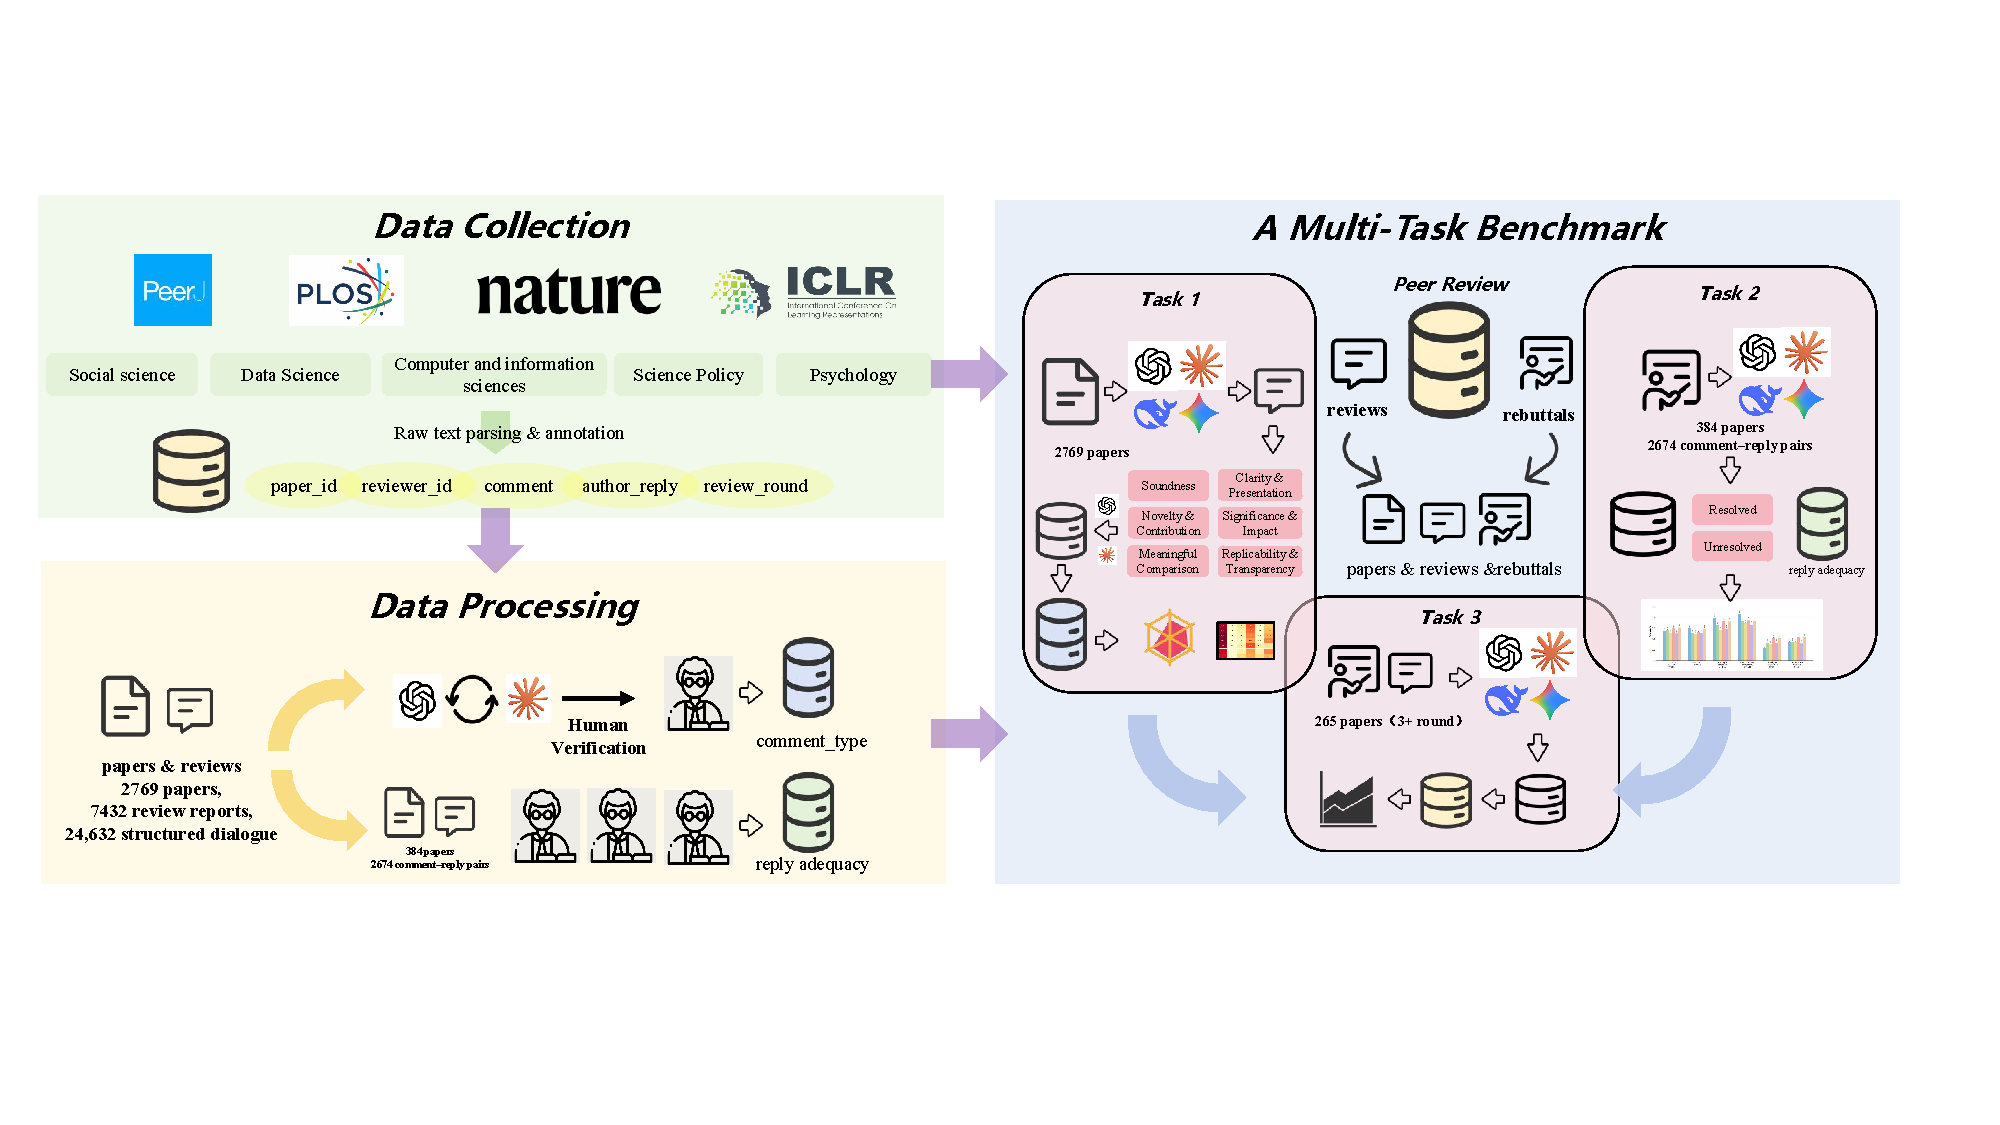
\includegraphics[width=\linewidth]{fig1.pdf}
\caption{Overview of the Multi-Task Benchmark Framework for LLM-based Peer Review.}
\label{fig:framework}
\end{figure}

\subsection{Evaluation Metrics}
\label{sec:metrics}

To comprehensively evaluate model performance, this study adopts multiple metrics. Coverage rate and round-level accept prediction rate assess the distributional coverage of review dimensions and the model's sensitivity to round-wise review progression, respectively. For binary decision tasks, Accuracy, Precision, Recall, F1 score, and Cohen's kappa are used to evaluate predictive performance and agreement with the reference labels beyond chance.

\subsubsection{Coverage rate}

In Task 1, the coverage rate quantifies the extent to which LLM-generated comments are distributed across the six categories in alignment with the human review baseline. This metric evaluates the allocation of model attention among review dimensions. For category $c$, coverage rate is defined as:
\begin{equation}
  \mathrm{Coverage}_c = \frac{n_c}{N}
  \label{eq:coverage}
\end{equation}
where $n_c$ denotes the number of comments assigned to category $c$, and $N$ denotes the total number of comments generated by the model. A coverage rate approximating the corresponding human proportion suggests the model's review focus is similar to that of human reviewers.

\subsubsection{Performance metrics for binary decision tasks}

The binary classification tasks used in the study were evaluated using Accuracy, Precision, Recall, F1 score, and Cohen's kappa.

\textbf{Accuracy} evaluates the proportion of correctly classified instances, indicating overall model performance as follows:
\begin{equation}
  \mathrm{Accuracy} = \frac{TP + TN}{TP + TN + FP + FN}
  \label{eq:acc}
\end{equation}
where $TP$, $TN$, $FP$, and $FN$ denote true positives, true negatives, false positives, and false negatives, respectively.

\textbf{Precision} measures the proportion of predicted positive instances that are actually positive, showing the reliability of positive predictions:
\begin{equation}
  \mathrm{Precision} = \frac{TP}{TP + FP}
  \label{eq:prec}
\end{equation}

\textbf{Recall} measures the proportion of actual positive instances that are correctly identified by the model:
\begin{equation}
  \mathrm{Recall} = \frac{TP}{TP + FN}
  \label{eq:rec}
\end{equation}

\textbf{F1 score} provides a balanced measure of positive-class identification performance:
\begin{equation}
  F_1 = \frac{2 \times \mathrm{Precision} \times \mathrm{Recall}}{\mathrm{Precision} + \mathrm{Recall}}
  \label{eq:f1}
\end{equation}

\textbf{Cohen's kappa} is further adopted to assess agreement between predicted and true labels while correcting for chance agreement, because Accuracy may overestimate model performance under class imbalance. It is defined as:
\begin{equation}
  \kappa = \frac{P_o - P_e}{1 - P_e}
  \label{eq:kappa}
\end{equation}
where $P_o$ is the observed agreement rate and $P_e$ is the expected agreement rate computed from the marginal distributions of predicted and true labels. A value of 0 indicates performance equivalent to random guessing, while a value of 1 indicates perfect agreement.

\subsubsection{Round-level accept prediction rate}

To assess whether the model captures the progression of peer review, we build on prior work that predicts acceptance decisions in peer review~\cite{ref40}. We define the round-level accept prediction rate as the proportion of accept predictions at each relative round. To make paper trajectories comparable, we index rounds by distance from the final round---such as Last, Round $-2$, and so on. For relative position $r$:
\begin{equation}
  \mathrm{APR}_r = \frac{\sum_{i=1}^{M_r} \mathbf{1}[\hat{y}_i = \mathrm{Accept}]}{M_r}
  \label{eq:accept-rate}
\end{equation}
where $M_r$ denotes the number of instances at relative round position $r$, and $\hat{y}_i$ denotes the predicted label for instance $i$. This metric is used to characterise whether the model produces an acceptance trajectory consistent with the underlying review process. Ideally, the model should keep a low Accept prediction rate in non-final rounds and increase the rate substantially in the final round.

%%======================================================================
\section{Task 1: Review Dimension Coverage}
\label{sec:task1}
%%======================================================================

\subsection{Experimental Setup}
\label{sec:t1-setup}

Each model generated a free-form peer-review report for all 2,769 papers, based solely on the manuscript text. No category labels, scoring rubrics, or structural constraints were imposed, simulating the open-ended conditions of human reviewers. The prompt directed each model to act as an expert reviewer, follow the target journal's format, examine all figures and tables, and give point-by-point commentary. This prompt was applied uniformly with GPT-4, GPT-4o, Claude Opus 4.6, Claude Sonnet 4.6, DeepSeek R1, and Gemini 3 Pro for consistent comparison.

All generated comments were classified using the Comment Type Taxonomy from Section~\ref{sec:data}, following the annotation protocol described earlier, with Claude Haiku 4.5 and GPT-4o as alignment annotators. The proportion in each category was calculated as its coverage rate and used as the main comparison metric, measuring each model's capacity to identify and address distinct comment types in peer review.

\subsection{Results}
\label{sec:t1-results}

\subsubsection{Overall Distribution of Critique Types}

Table~\ref{tab:distribution} reports the distribution of six large language models and human reviewers across six categories of critical dimensions. Soundness dominates across all sources: it accounts for 42.70\% of human reviewer feedback, while the six models range from 37.29\% to 46.60\%---a deviation from the human baseline that remains largely within 5 percentage points. Clarity \& Presentation and Replicability \& Transparency are also dimensions with high prevalence, at 29.21\% and 14.60\%, respectively, in the human baseline; however, the distribution across models within these two categories shows relatively distinct patterns. The remaining three categories generally account for a smaller proportion of feedback but present more distinctive distributional characteristics. Novelty \& Contribution remains low for both humans and models ($\leq 2.25\%$); moreover, the models generally fall below the human baseline in this category, suggesting that, within the context of this benchmark, they pay relatively insufficient attention to novelty. Significance \& Impact accounts for only 2.25\% of human critiques; however, the proportion for some models is notably higher---up to 11.15\%---indicating that, compared to human reviewers, models tend to place greater emphasis on impact-related issues. In contrast, Meaningful Comparison accounts for 8.99\% of human reviewer feedback, whereas model coverage ranges from 3.48\% to 11.86\%, with 4 of the 6 models falling below the human level.

\begin{table}[htbp]
\centering
\caption{Distribution of peer review comment types across six LLMs and human reviewers.}
\label{tab:distribution}
\resizebox{\linewidth}{!}{%
\begin{tabular}{l r rr rr rr rr rr rr}
\toprule
 &
 &
 \multicolumn{2}{c}{\textbf{Soundness}} &
 \multicolumn{2}{c}{\textbf{Novelty \& Contrib.}} &
 \multicolumn{2}{c}{\textbf{Meaningful Comp.}} &
 \multicolumn{2}{c}{\textbf{Clarity \& Pres.}} &
 \multicolumn{2}{c}{\textbf{Significance \& Impact}} &
 \multicolumn{2}{c}{\textbf{Replicability \& Trans.}} \\
\cmidrule(lr){3-4}\cmidrule(lr){5-6}\cmidrule(lr){7-8}\cmidrule(lr){9-10}\cmidrule(lr){11-12}\cmidrule(lr){13-14}
\textbf{Model} & \textbf{Total} &
 $n$ & \% &
 $n$ & \% &
 $n$ & \% &
 $n$ & \% &
 $n$ & \% &
 $n$ & \% \\
\midrule
Human (baseline) & 24\,632 &
 10\,517 & 42.70 &
   554 & 2.25 &
  2\,214 & 8.99 &
  7\,196 & 29.21 &
    554 & 2.25 &
  3\,597 & 14.60 \\
Claude Opus 4.6  & 25\,186 &
 11\,347 & 45.05 &
   446 & 1.77 &
  1\,689 & 6.71 &
  6\,945 & 27.57 &
   513 & 2.04 &
  4\,246 & 16.86 \\
Claude Sonnet 4.6 & 28\,507 &
 13\,285 & 46.60 &
   401 & 1.41 &
  1\,546 & 5.42 &
  7\,165 & 25.13 &
   721 & 2.53 &
  5\,389 & 18.90 \\
DeepSeek R1       & 18\,543 &
  8\,580 & 46.27 &
   277 & 1.49 &
    645 & 3.48 &
  3\,978 & 21.45 &
   397 & 2.14 &
  4\,666 & 25.16 \\
Gemini 3 Pro      & 14\,945 &
  6\,642 & 44.44 &
   304 & 2.03 &
    950 & 6.36 &
  4\,536 & 30.35 &
  1\,107 & 7.41 &
  1\,406 &  9.41 \\
GPT-4             & 19\,843 &
  7\,731 & 38.96 &
   345 & 1.74 &
  1\,125 & 5.67 &
  4\,312 & 21.73 &
  1\,398 & 7.05 &
  4\,932 & 24.86 \\
GPT-4o            & 16\,329 &
  6\,089 & 37.29 &
   289 & 1.77 &
  1\,937 & 11.86 &
  3\,216 & 19.70 &
  1\,821 & 11.15 &
  2\,977 & 18.23 \\
\bottomrule
\end{tabular}}
\end{table}

\subsubsection{Differences Across Models}

Figure~\ref{fig:radar} presents the critique-type profiles of the six models in a $2\times 3$ radar-chart panel, with the human baseline overlaid as a grey dashed reference. In terms of polygon overlap, Claude Opus 4.6 and Claude Sonnet 4.6 exhibit the closest alignment with the human baseline, deviating by fewer than five percentage points on the three dominant dimensions---Soundness, Clarity \& Presentation, and Replicability \& Transparency. DeepSeek R1 expands markedly along the Replicability \& Transparency axis (25.16\% vs.\ 14.60\% for humans) while contracting on Meaningful Comparison (3.48\% vs.\ 8.99\%), reflecting a disproportionate focus on reproducibility at the expense of scholarly positioning. Gemini 3 Pro shows slightly elevated Clarity \& Presentation coverage (30.35\% vs.\ 29.21\%), but records the lowest Replicability \& Transparency among all models (9.41\% vs.\ 14.60\%), with its polygon visibly contracting along the transparency axis. Both GPT-4 and GPT-4o deviate substantially from the human baseline on Significance \& Impact (7.05\% and 11.15\%, respectively, well above the human baseline of 2.25\%). GPT-4o diverges further on Meaningful Comparison (11.86\% vs.\ 8.99\%) and registers the lowest Soundness (37.29\%) and Clarity \& Presentation (19.70\%) among all models. This distributional profile suggests relatively greater emphasis on macro-level impact and literature comparison, accompanied by less sustained attention to methodological detail and writing quality.

\begin{figure}[htbp]
\centering
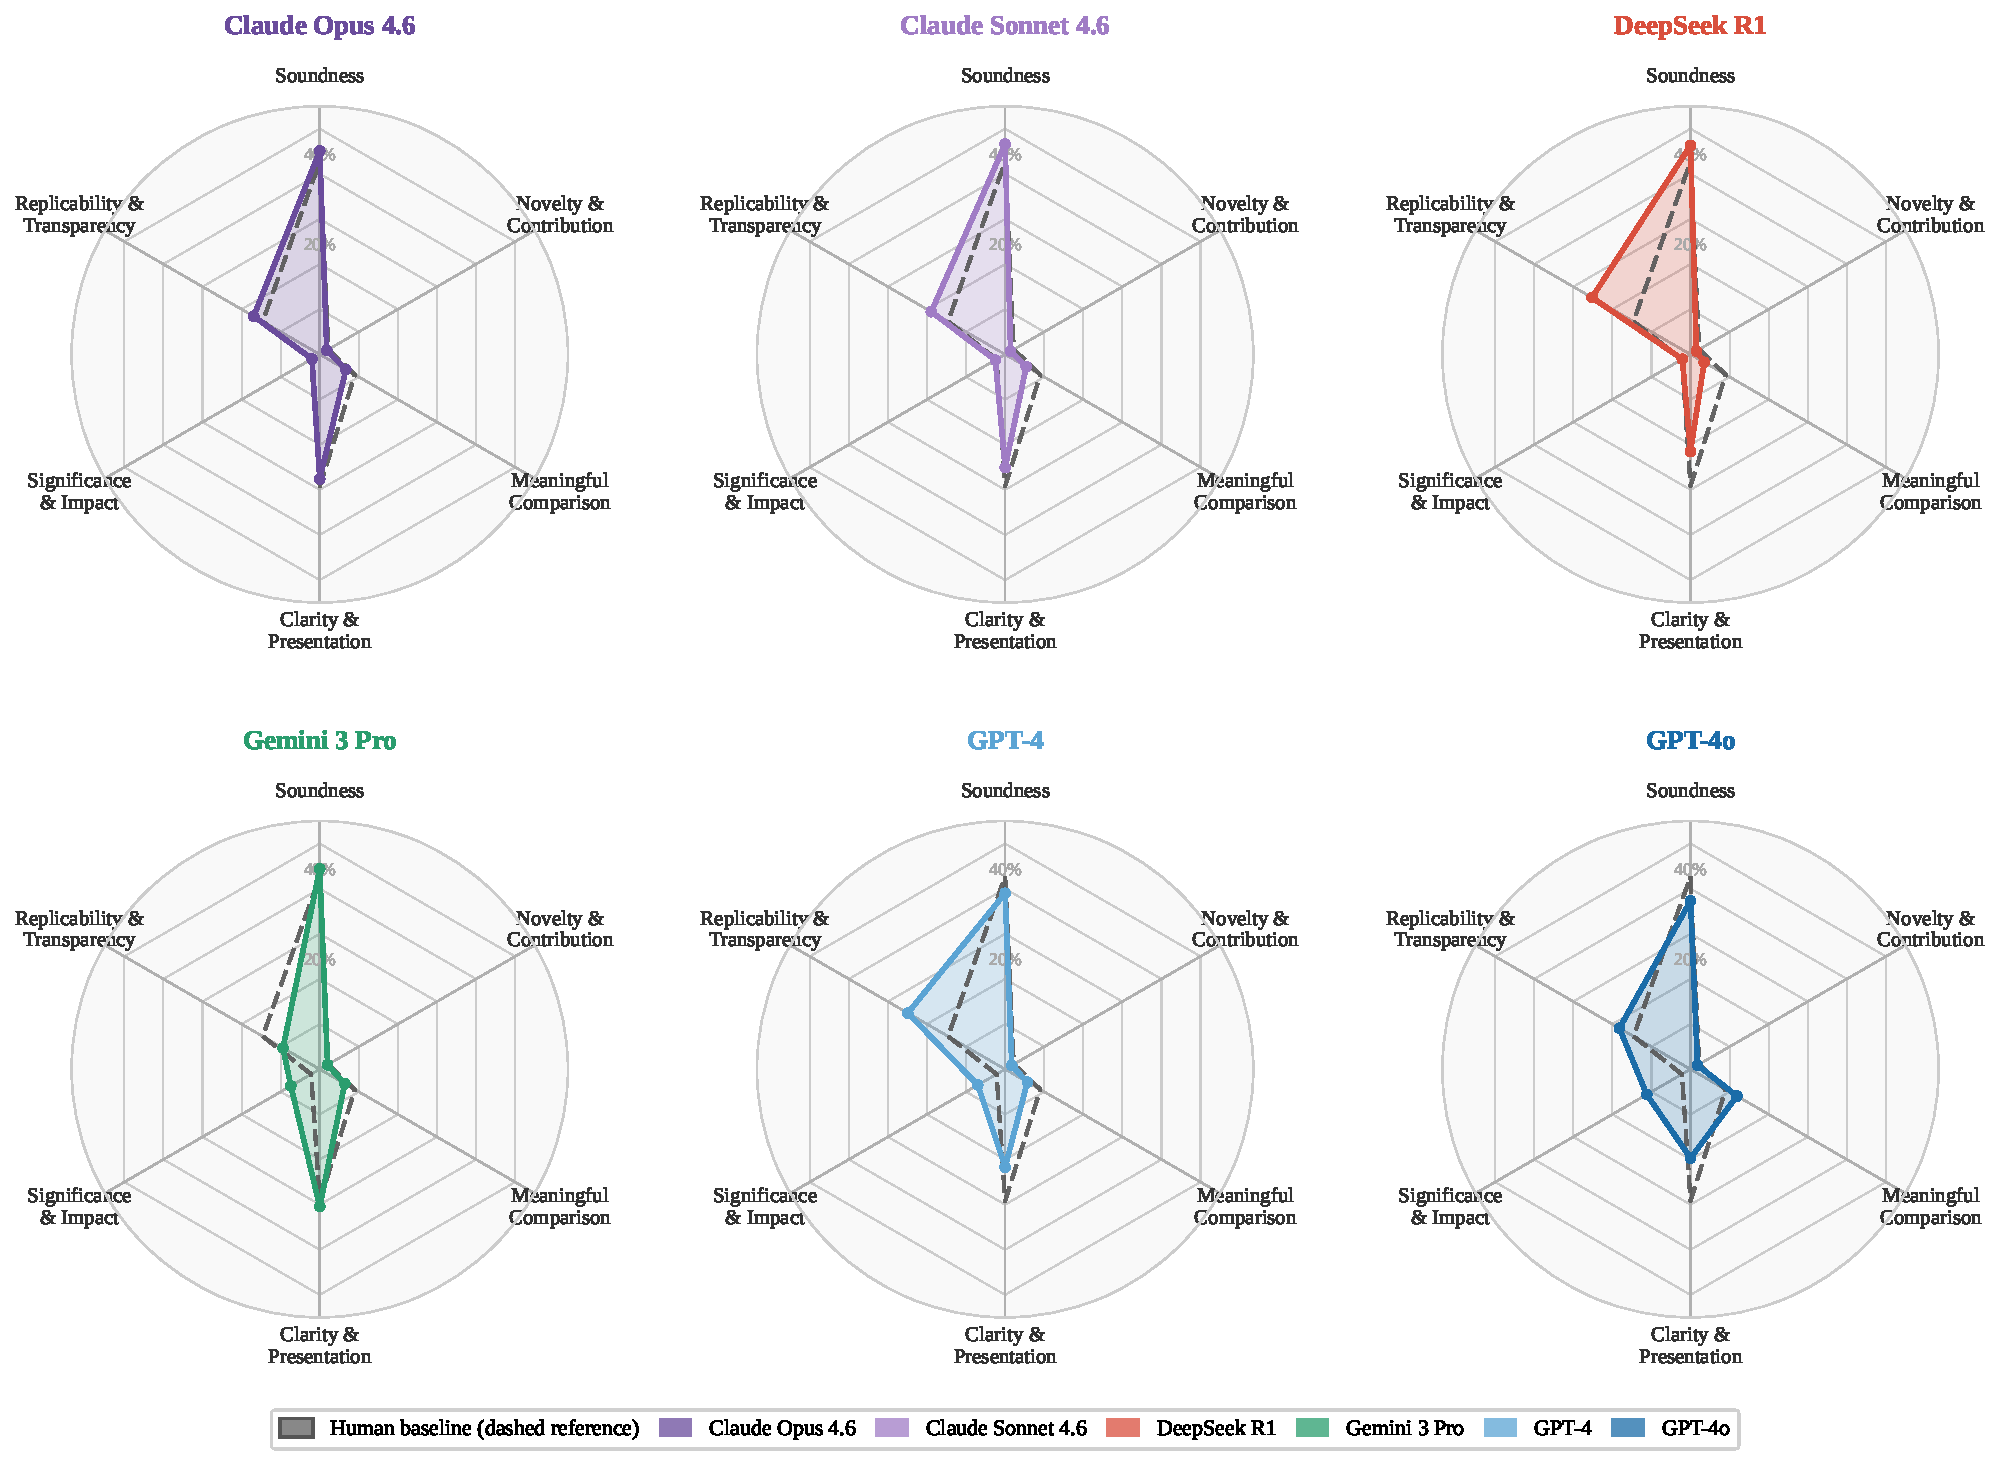
\includegraphics[width=\linewidth]{fig2.pdf}
\caption{Radar chart comparison of comment category coverage between each LLM model and the human reviewer baseline across six evaluation dimensions.}
\label{fig:radar}
\end{figure}

Figure~\ref{fig:heatmap} shows a heatmap of the model-by-category coverage matrix, with colour intensity ranging from light yellow (low coverage) to deep red (high coverage). The human baseline is placed in the top row for reference. The Soundness column remains dark across all rows, confirming its dominance as the primary critique category. By contrast, Novelty \& Contribution stays consistently light, indicating its limited presence at the rebuttal stage. The largest inter-model differences appear in three dimensions. In Replicability \& Transparency, DeepSeek R1 (25.16\%) and Gemini 3 Pro (9.41\%) differ by more than 15 percentage points and deviate from the human baseline (14.60\%) in opposite directions. In Significance \& Impact, GPT-4o (11.15\%) stands out as a much darker cell in an otherwise light column, reaching nearly five times the human proportion (2.25\%). In Meaningful Comparison, GPT-4o (11.86\%) and DeepSeek R1 (3.48\%) form a clear contrast, with GPT-4o above and DeepSeek R1 below the human baseline (8.99\%). Together, these colour differences highlight systematic variation in the emphasis placed on reviews across models.

\begin{figure}[htbp]
\centering
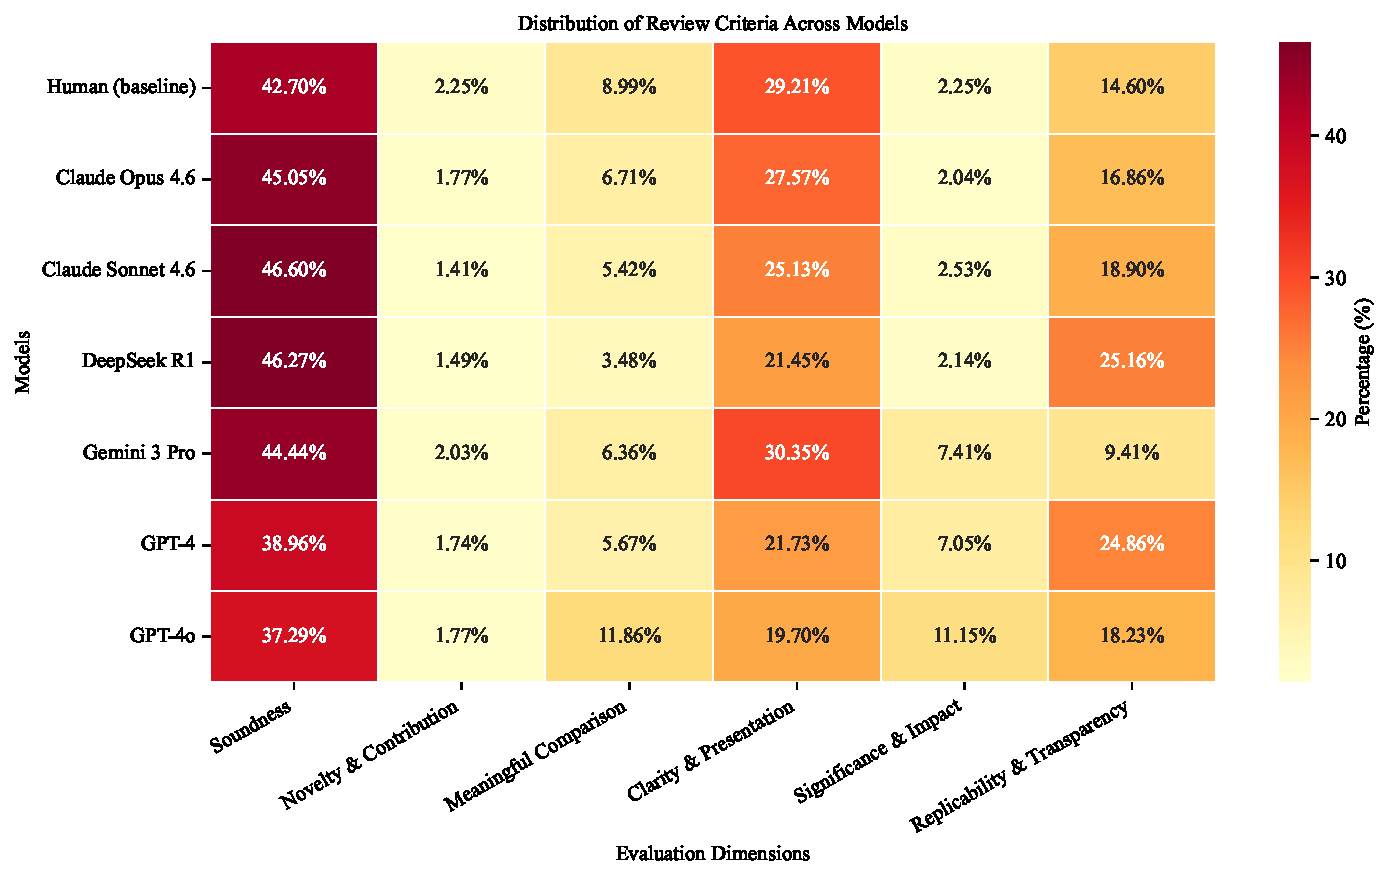
\includegraphics[width=\linewidth]{fig3.pdf}
\caption{Heatmap of comment category coverage rates ($\%$) by model and category; the human baseline row is highlighted with a bold border.}
\label{fig:heatmap}
\end{figure}

%%======================================================================
\section{Task 2: Reply Resolution Judgment}
\label{sec:task2}
%%======================================================================

\subsection{Experimental Setup}
\label{sec:t2-setup}

This task evaluates whether LLMs can judge whether a reviewer's concern is reflected as resolved in a comment--reply pair. The evaluation is based on the reply resolution annotations described in Section~\ref{sec:data}, using the balanced subset of 2,674 comment--reply pairs (1,640 Resolved and 1,034 Unresolved) drawn from 384 papers. The experimental procedure was as follows. For each comment--reply pair, the original reviewer comment and the corresponding author reply were used as input to construct a standardised prompt. The prompt instructed the model to act as a peer-review expert, assess whether the reviewer's concern was resolved based on the author's reply, and return a binary label: \textit{Resolved} or \textit{Unresolved}. The input included no access to the full manuscript text or review information from other rounds; the model's judgment relied entirely on the textual exchange between a single criticism and its corresponding reply. All 2,674 pairs were submitted to six models---GPT-4, GPT-4o, Claude Opus, Claude Sonnet, DeepSeek R1, and Gemini 3 Pro---and the resulting judgments were compared against human-annotated ground truth for evaluation.

\subsection{Results}
\label{sec:t2-results}

Table~\ref{tab:task2} reports the performance of each model on the reply resolution judgment task. Accuracy ranges from 0.506 (DeepSeek R1) to 0.839 (Gemini 3 Pro). However, Cohen's $\kappa$ values across all models remain below 0.1, indicating negligible agreement with the ground truth beyond chance. Gemini 3 Pro achieves the highest accuracy but the lowest $\kappa$ (0.002), as its predictions are overwhelmingly dominated by the Resolved label. GPT-4 obtains the highest $\kappa$ (0.093), while GPT-4o yields the highest Recall (0.533) and F1 (0.268) for the Unresolved class. Claude Opus ranks second in accuracy (0.735) and highest in Precision (0.187), though with comparatively lower Recall (0.311). Taken together, these results suggest that current LLMs have limited ability to align with trajectory-based reply-resolution labels in this benchmark setting.

\begin{table}[htbp]
\centering
\caption{Performance of LLMs on the reply resolution judgment task (Unresolved as positive class).}
\label{tab:task2}
\begin{tabular}{l ccccc}
\toprule
\textbf{Model} & \textbf{Accuracy} & \textbf{Cohen's $\kappa$} & \textbf{Precision} & \textbf{Recall} & \textbf{F1} \\
\midrule
Gemini 3 Pro  & 0.839 & 0.002 & 0.133 & 0.044 & 0.067 \\
GPT-4         & 0.695 & 0.093 & 0.186 & 0.400 & 0.254 \\
GPT-4o        & 0.622 & 0.092 & 0.179 & 0.533 & 0.268 \\
Claude Sonnet & 0.640 & 0.066 & 0.167 & 0.444 & 0.242 \\
DeepSeek R1   & 0.506 & 0.032 & 0.146 & 0.578 & 0.233 \\
Claude Opus   & 0.735 & 0.085 & 0.187 & 0.311 & 0.233 \\
\bottomrule
\end{tabular}
\end{table}

Figure~\ref{fig:cat-acc} presents model accuracy disaggregated by review category. All models achieve their highest accuracy on Replicability \& Transparency (0.667--0.867) and Meaningful Comparison (0.573--0.792). Accuracy declines markedly for Novelty \& Contribution (0.231--0.421) and Significance \& Impact (0.317--0.438), remaining below 0.45 across all models in both categories. The two largest categories---Clarity \& Presentation ($n = 1{,}073$) and Soundness ($n = 860$)---fall in an intermediate range, with accuracy between 0.495 and 0.613. Notably, Claude Sonnet and Claude Opus exhibit relatively consistent performance across categories, including the two in which other models struggle most.

\begin{figure}[htbp]
\centering
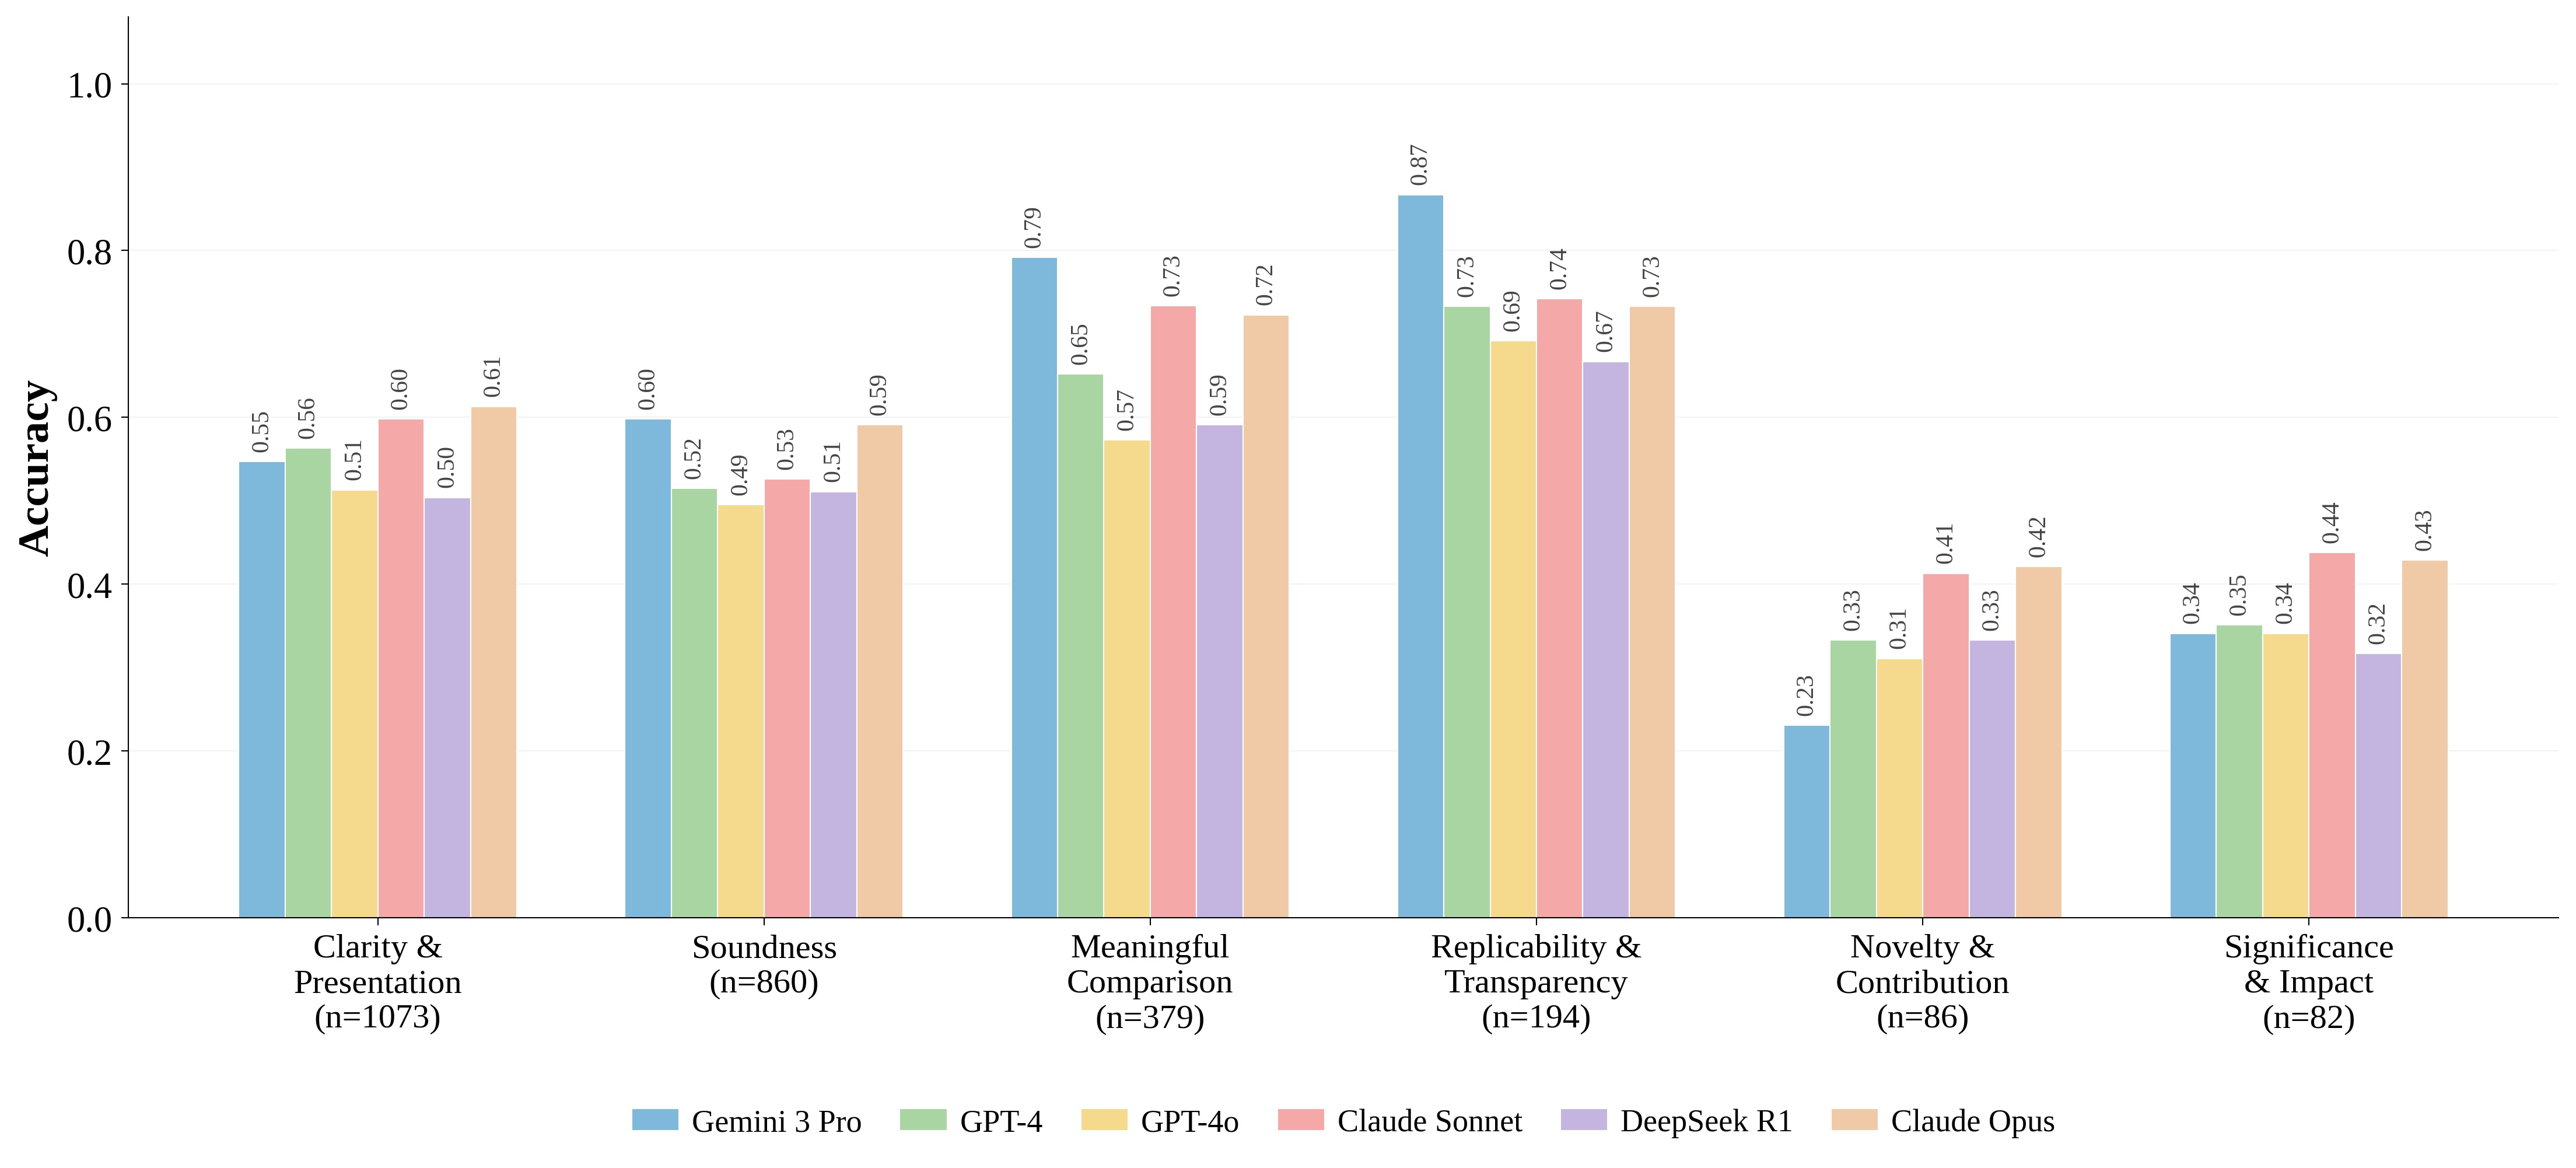
\includegraphics[width=\linewidth]{fig4.jpg}
\caption{Model accuracy on reply resolution judgment disaggregated by review category.}
\label{fig:cat-acc}
\end{figure}

Figure~\ref{fig:error-dir} exposes the distinct patterns driving each model's judgments and error directionality. Opus leads with the highest correct rate (62.5\%), but its pronounced tendency for over-optimistic errors (27.3\%) signals a consistent misclassification of unresolved issues as resolved. DeepSeek R1, in stark contrast, produces the greatest share of over-pessimistic errors (34.1\%), routinely mislabeling resolved issues as unresolved. GPT-4o follows closely, with 32.8\% of its errors being over-pessimistic. GPT-4 and Claude Sonnet show rare equilibrium, with neither error type surpassing 23.4\%. These results reveal forceful directional biases: Gemini 3 Pro and Claude Opus tilt toward leniency, while DeepSeek R1 and GPT-4o sharply favor excessive skepticism.

\begin{figure}[htbp]
\centering
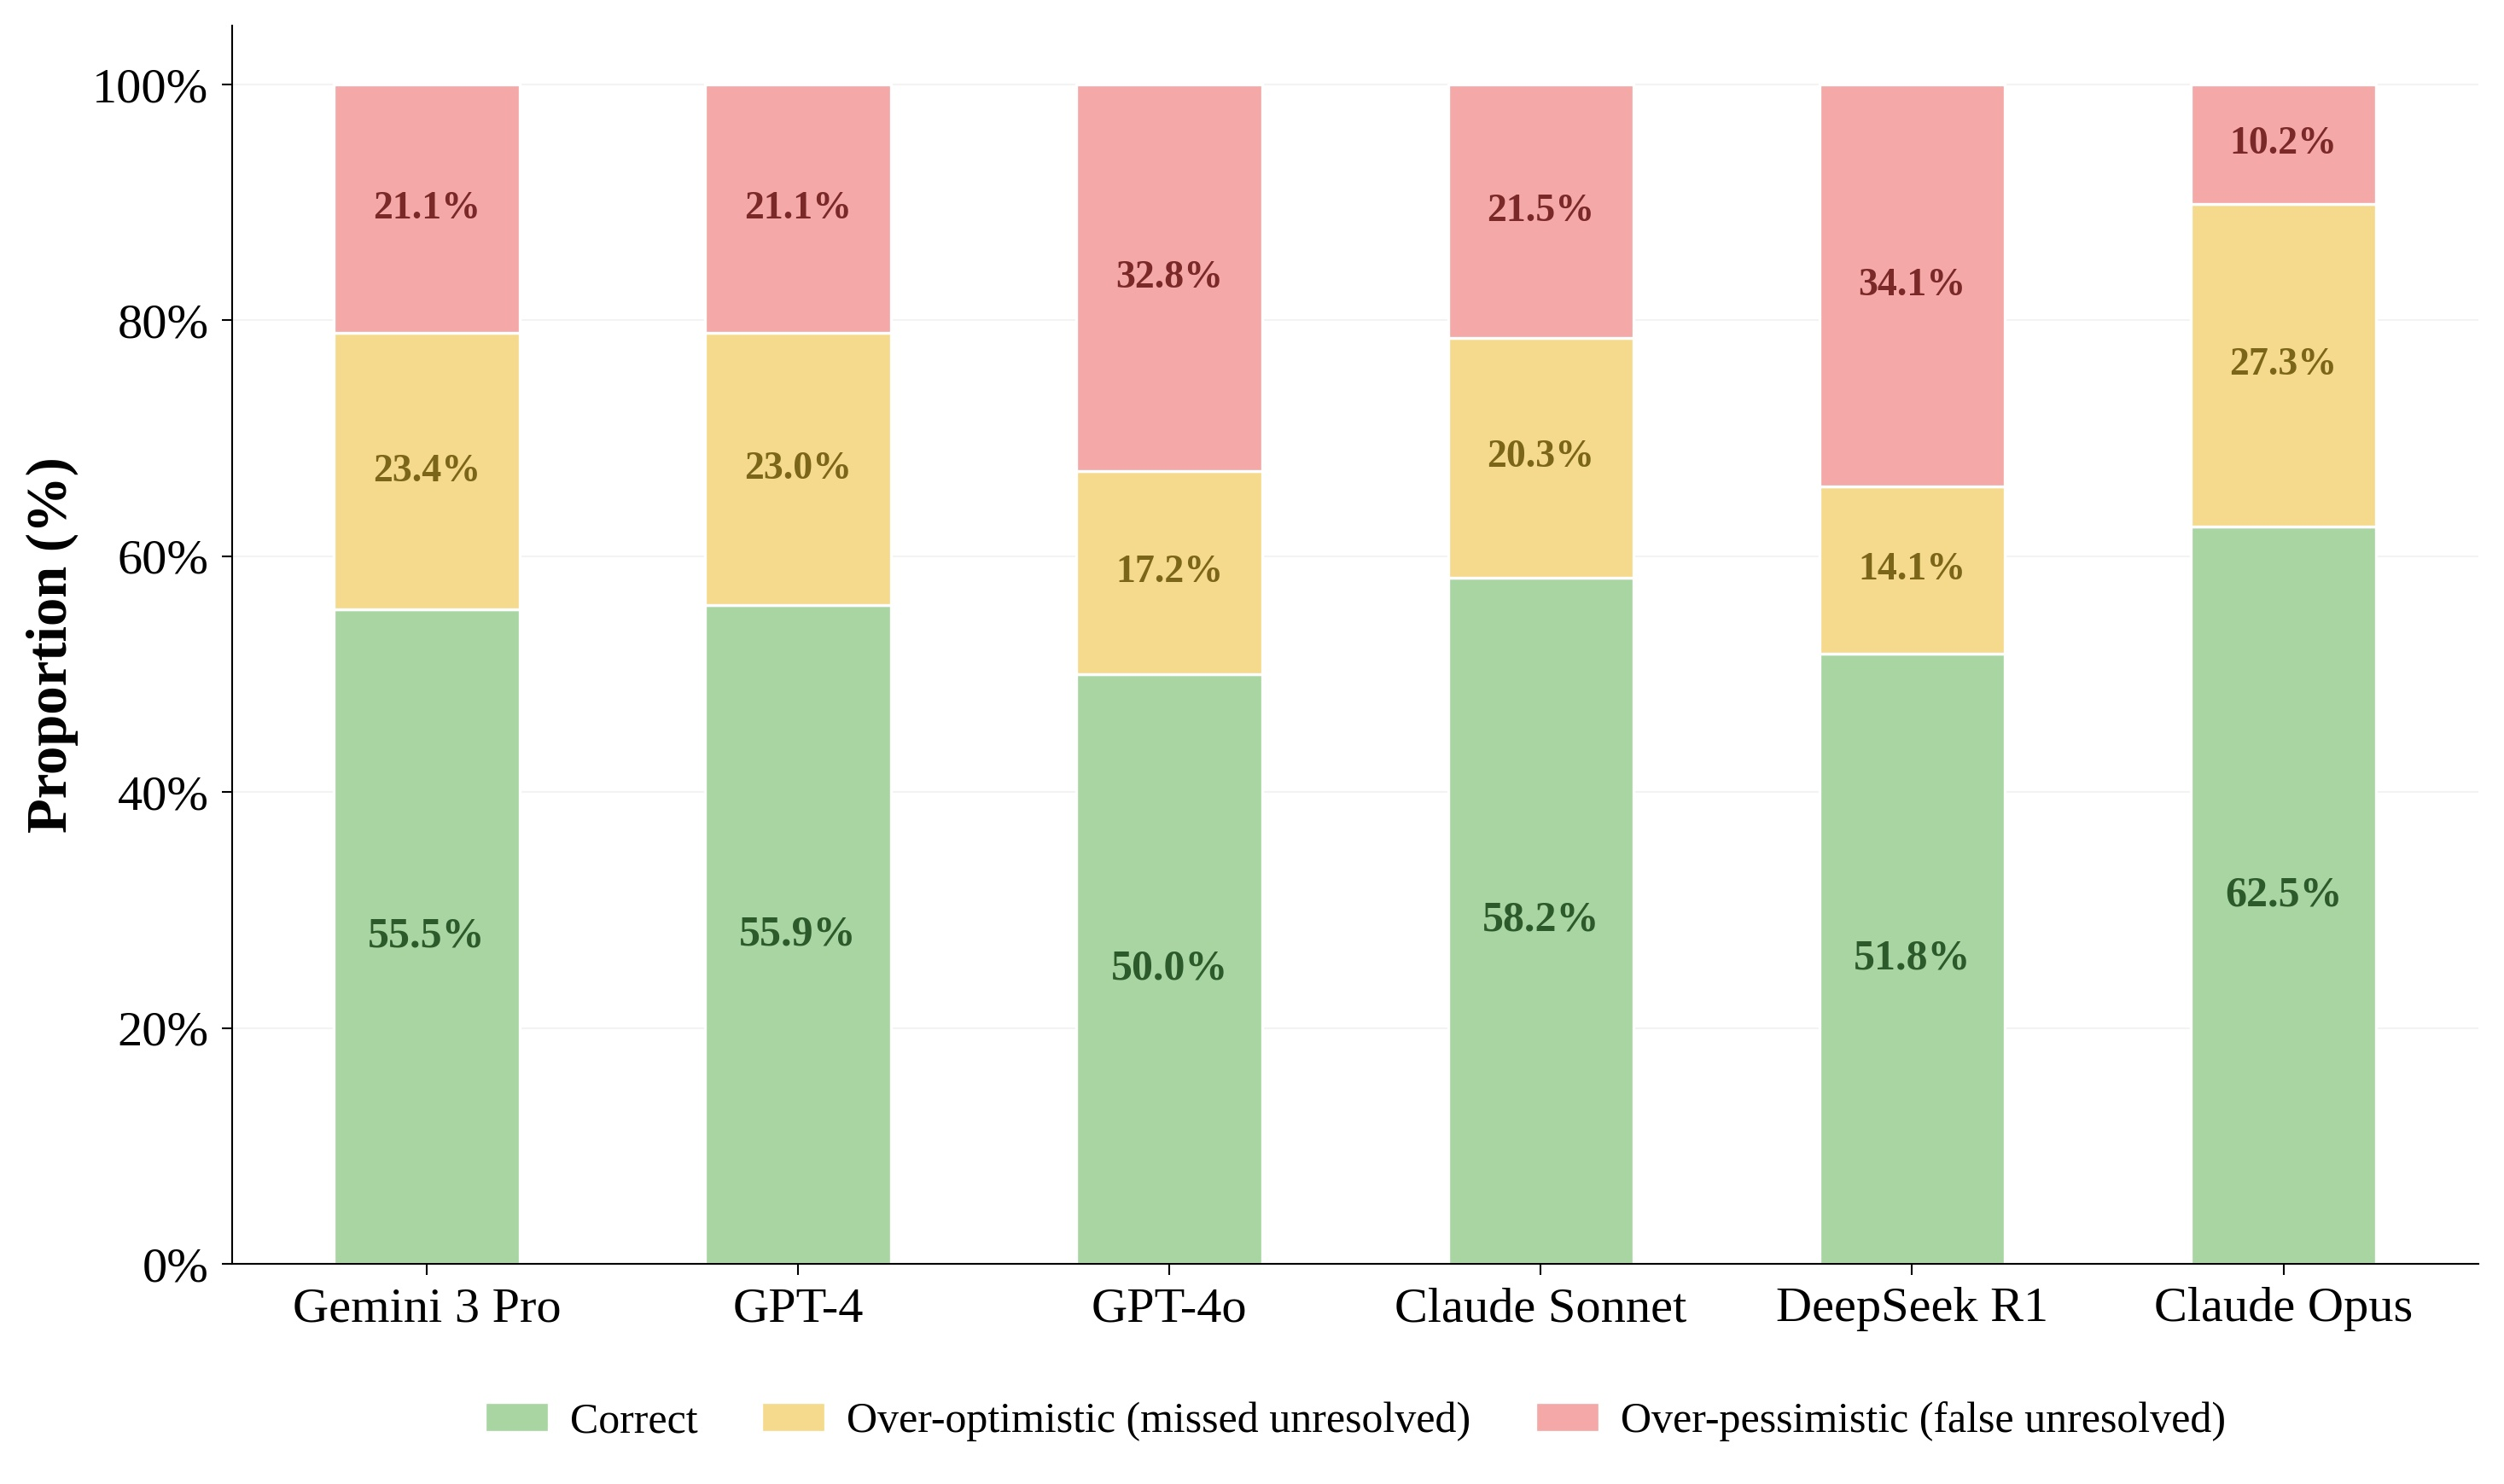
\includegraphics[width=\linewidth]{fig5.jpg}
\caption{Judgment composition and error directionality of each model on the reply resolution judgment task.}
\label{fig:error-dir}
\end{figure}

%%======================================================================
\section{Task 3: Round-Level Acceptability Judgment}
\label{sec:task3}
%%======================================================================

\subsection{Experimental Setup}
\label{sec:t3-setup}

Task 3 further examines whether LLMs can make round-level acceptability judgments given complete review information. This task requires models to simultaneously weigh the severity of reviewer criticisms, the extent to which author replies address those concerns, and the overall quality of the revised manuscript, thereby producing a holistic round-level judgment. We selected all 265 papers containing three or more complete review rounds from the dataset. For each review round, the model receives three inputs: (1) all reviewer criticisms from that round, (2) the corresponding author rebuttals, and (3) the full text of the revised manuscript. The model is then required to produce a binary classification: \textit{Accept} or \textit{Needs Revision}. Each round is evaluated independently, with no information about subsequent rounds provided.

The gold standard is derived from each paper's actual editorial trajectory. For all non-final rounds, the ground-truth label is ``Needs Revision''; for the final round, the label is ``Accept''. This operationalization approximates round-level acceptance status as reflected in the observed review trajectory. Notably, the resulting label distribution is inherently imbalanced: only the final round of each paper receives an Accept label, while all preceding rounds are labeled Needs Revision.

To enable meaningful aggregation across papers with varying numbers of review rounds, we index rounds by their relative distance from the final round: the last round is designated Last Round, the penultimate round Round $-2$, the antepenultimate round Round $-3$, and so forth. Six models---GPT-4, GPT-4o, Claude Opus 4.6, Claude Sonnet 4.6, DeepSeek R1, and Gemini 3 Pro---are evaluated under identical conditions.

\subsection{Results}
\label{sec:t3-results}

Table~\ref{tab:task3} reports the binary classification performance of each model across all rounds. All six models achieved accuracy above 0.70, with Claude Opus attaining the highest (0.789) and GPT-4o the lowest (0.702). However, Cohen's $\kappa$ ranged from only 0.218 (GPT-4o) to 0.432 (Claude Opus), indicating that agreement beyond chance remains limited despite ostensibly reasonable accuracy. Even the best-performing model falls within the ``moderate agreement'' range, suggesting that round-level acceptability judgment remains challenging for current LLMs under this benchmark setting. Precision and recall, computed with Accept as the positive class, follow a consistent ranking: Claude Opus leads on both metrics (Precision = 0.714, Recall = 0.658), while GPT-4o scores lowest (Precision = 0.548, Recall = 0.526). Claude Sonnet, GPT-4, and DeepSeek R1 occupy the middle tier, with F1 scores between 0.605 and 0.642.

Notably, these accuracy figures are partly inflated by the label imbalance inherent in the task design. Because non-final rounds (labeled Needs Revision) substantially outnumber final rounds (labeled Accept), a na\"{\i}ve classifier that uniformly predicts Needs Revision would achieve non-trivial accuracy. The modest $\kappa$ values confirm that much of the observed accuracy reflects this baseline bias rather than genuine predictive capability.

\begin{table}[htbp]
\centering
\caption{Overall performance on accept/revise decision (Accept as positive class).}
\label{tab:task3}
\begin{tabular}{l ccccc}
\toprule
\textbf{Model} & \textbf{Accuracy} & \textbf{Cohen's $\kappa$} & \textbf{Precision} & \textbf{Recall} & \textbf{F1} \\
\midrule
Claude Opus 4.6   & 0.789 & 0.432 & 0.714 & 0.658 & 0.685 \\
Claude Sonnet 4.6 & 0.754 & 0.371 & 0.652 & 0.632 & 0.642 \\
GPT-4             & 0.737 & 0.348 & 0.636 & 0.605 & 0.620 \\
DeepSeek R1       & 0.728 & 0.322 & 0.618 & 0.592 & 0.605 \\
Gemini 3 Pro       & 0.726 & 0.274 & 0.583 & 0.553 & 0.567 \\
GPT-4o            & 0.702 & 0.218 & 0.548 & 0.526 & 0.537 \\
\bottomrule
\end{tabular}
\end{table}

Figure~\ref{fig:round-curve} illustrates the predictions made by each model at every relative round position. The ideal predictive pattern for a model would be to predict ``Needs Revision'' (0\% acceptance rate) for all non-final rounds, and then switch to predicting ``Accept'' (100\% acceptance rate) in the final round. None of the six models approached this ideal pattern. By Round $-3$, all models already exhibited a certain acceptance rate---ranging from 10.5\% (Claude Opus) to 24.9\% (DeepSeek R1)---indicating that, even after multiple rounds of revision, the models still tended to deem manuscripts acceptable. Among them, Claude Opus was the most conservative, while the acceptance rates for the remaining models ranged from 18\% to 25\%. In Round $-2$, the acceptance rates for all models rose---ranging from 22.4\% (Claude Opus) to 42.1\% (GPT-4o)---and the disparities between the models widened significantly. The Claude models maintained relatively restrained prediction rates (22.4\% and 28.9\%, respectively), whereas GPT-4o and DeepSeek R1 exceeded 39\%. In the final round, the predicted acceptance rates for the various models ranged from 62.5\% (GPT-4o) to 84.2\% (Claude Opus). None of the models exceeded 85\%, indicating that they still produced substantial misclassifications. Claude Opus exhibited a curve that most closely resembled human patterns, suggesting it is the most sensitive to the progress of revisions. Conversely, GPT-4o displayed the flattest curve---rising only from 21.8\% to 62.5\%---reflecting its limited ability to distinguish between rounds that still require revision and those that are ready for acceptance.

\begin{figure}[htbp]
\centering
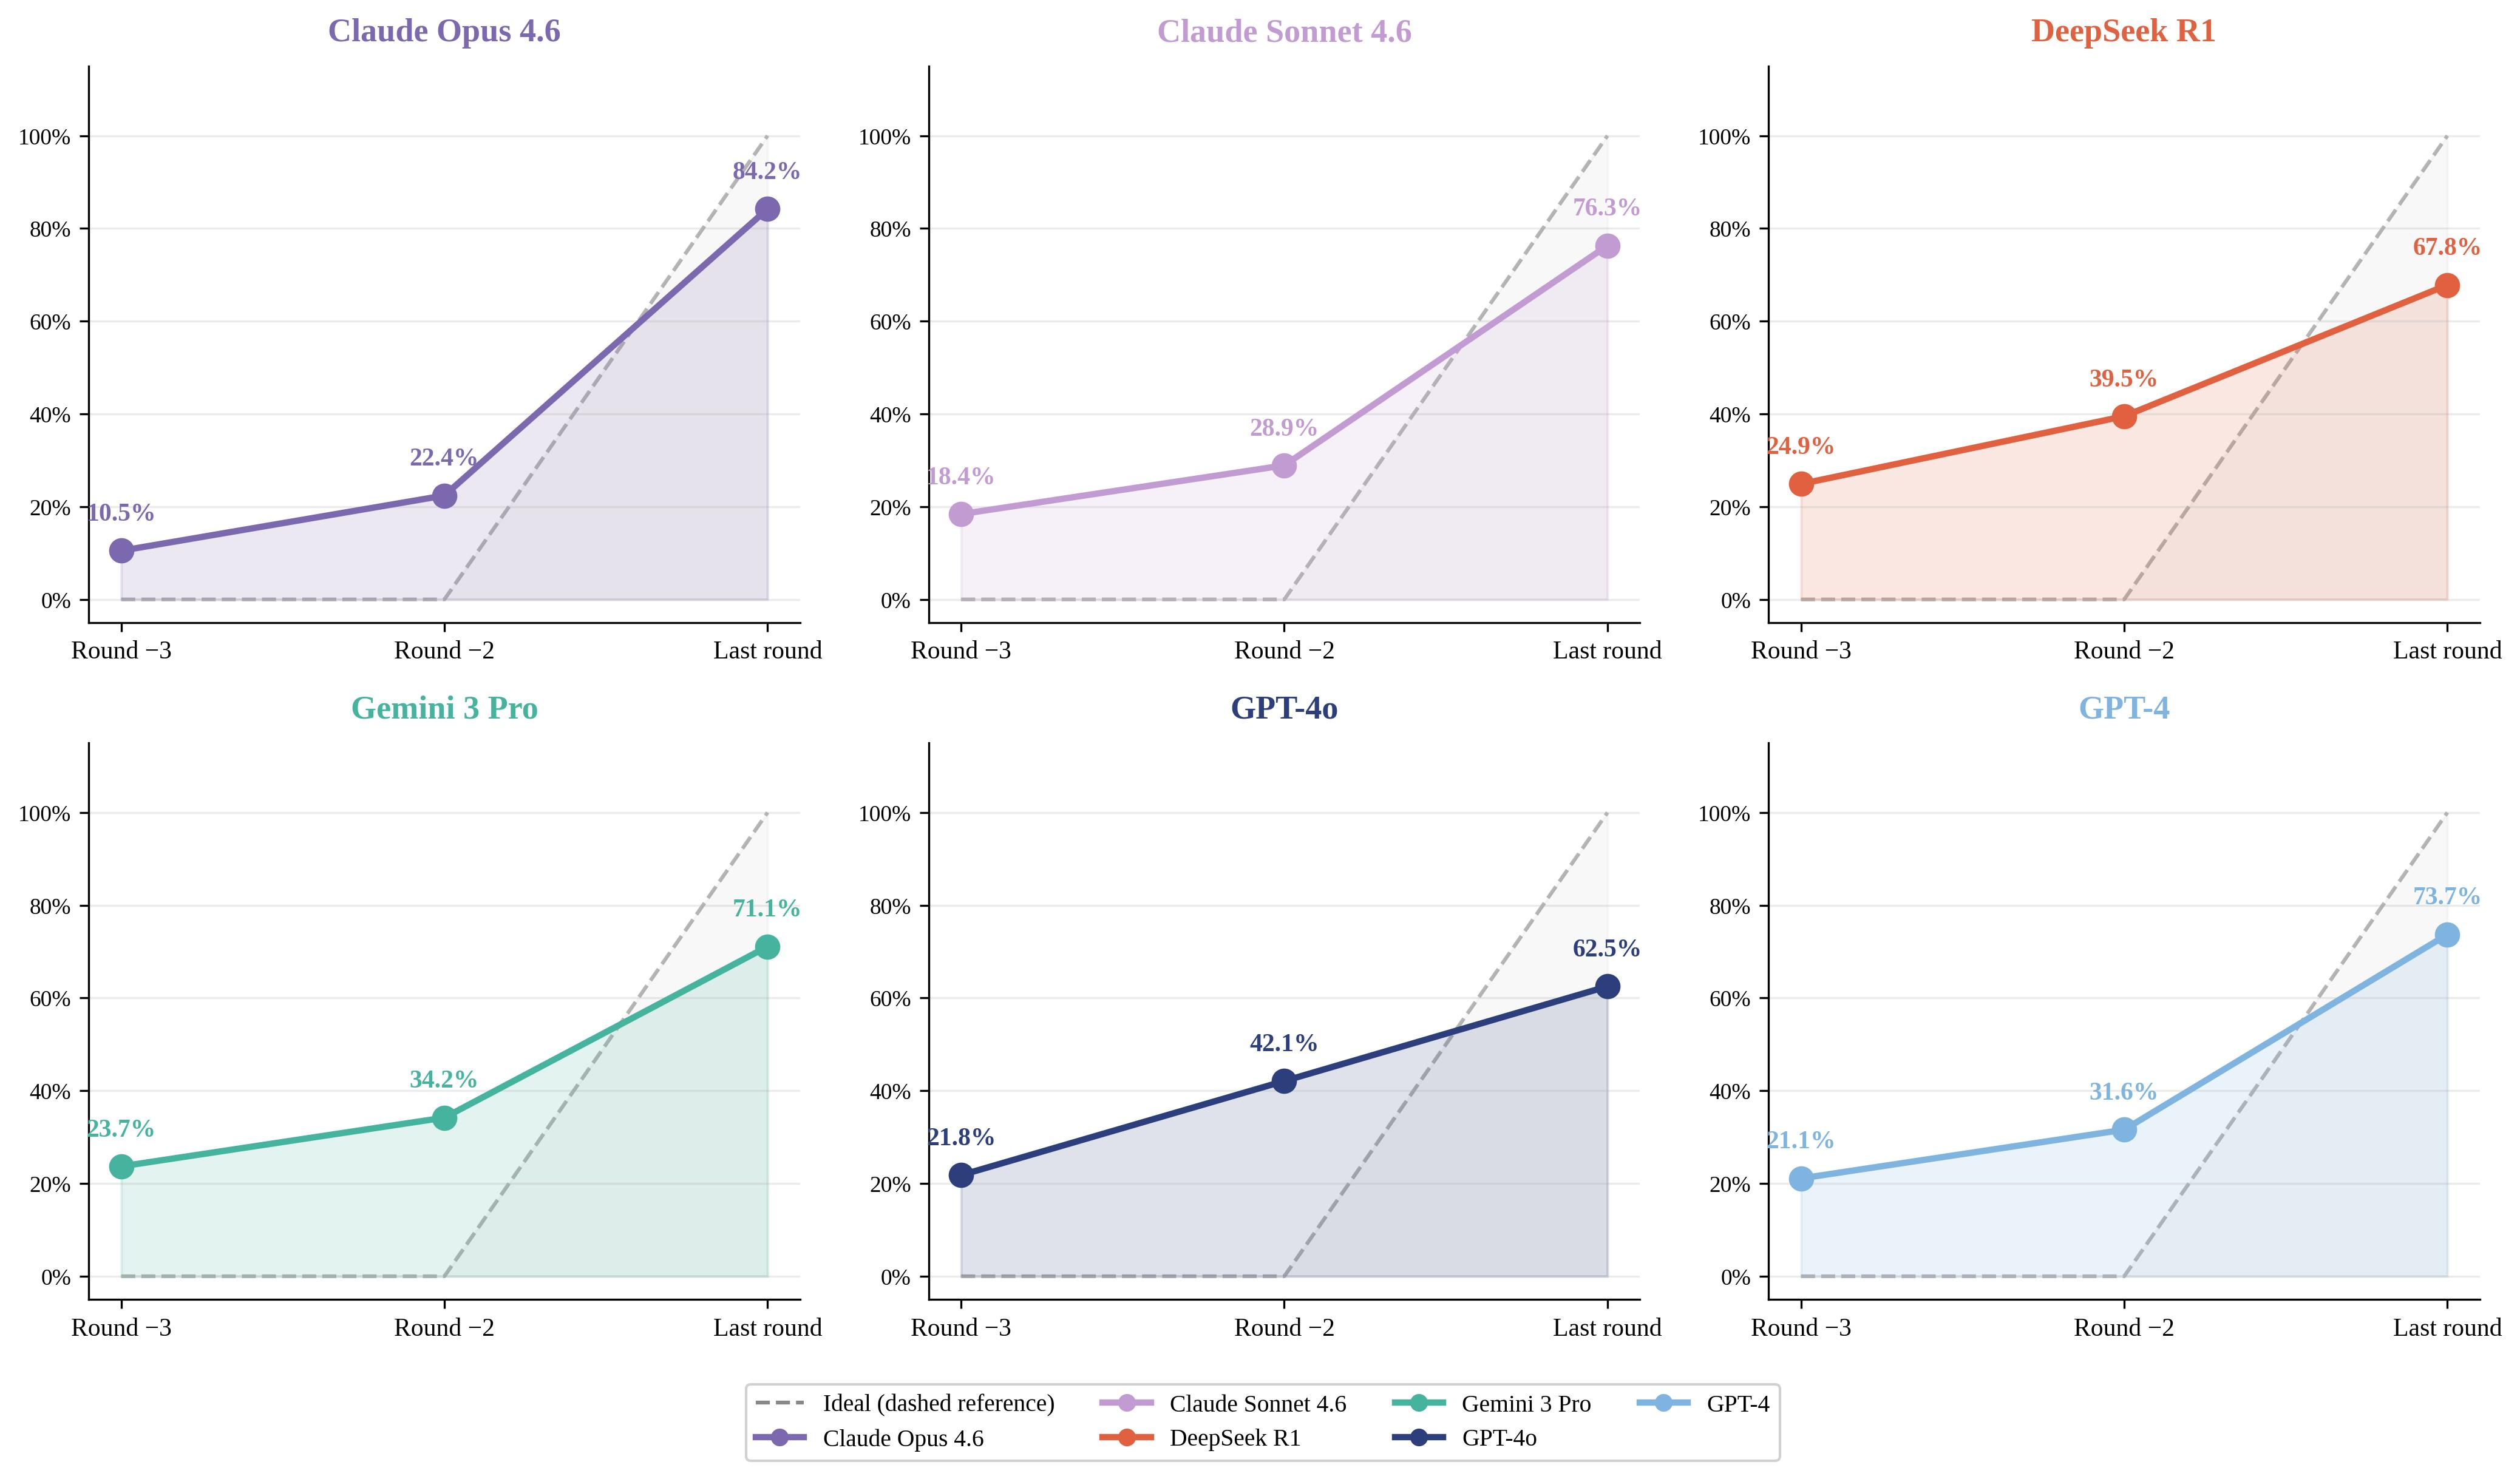
\includegraphics[width=\linewidth]{fig6.jpg}
\caption{Accept prediction rate by relative round position for each model. The dashed grey line represents the ideal pattern (0\% at non-final rounds, 100\% at the last round).}
\label{fig:round-curve}
\end{figure}

%%======================================================================
\section{Discussion}
\label{sec:discussion}
%%======================================================================

Evaluating six frontier LLMs across three open peer review tasks on our benchmark yields critical insights into their reasoning patterns, evaluative judgment, and task-specific limitations within the peer review process. This section examines two interrelated dimensions: (1) how model performance varies across tasks and what this reveals about the compound nature of peer review competence (Section~\ref{sec:task-var}), and (2) how models differ from one another in their evaluative tendencies, systematic biases, and task-specific suitability (Section~\ref{sec:model-var}).

\subsection{Performance Variation Across Tasks}
\label{sec:task-var}

Our multi-task evaluation reveals that LLMs do not degrade uniformly across open peer review tasks but instead exhibit a clear capability gradient. Models approximate human reviewers' macro-level distribution reasonably well in review dimension coverage, yet their performance falls off sharply in author reply resolution judgment and round-level acceptability judgment. Current LLMs are thus not devoid of peer review competence. Rather, that competence is concentrated in local judgments anchored to surface textual cues, and erodes once a task requires integrative reasoning across review comments, author responses, manuscript revisions, and round progression.

In Task 1, most models reproduce human reviewers' attention to core dimensions, with especially close alignment on Soundness. This echoes Shin et al.\ (2025), who report that LLMs and human reviewers alike treat technical validity as a primary focus~\cite{ref26}. Yet such alignment reflects the detection of overt methodological issues, not the simulation of holistic scholarly evaluation. All models fall below human coverage on Novelty \& Contribution, consistent with prior evidence on LLMs' weakness in novelty assessment~\cite{ref41,ref42}. With the exception of GPT-4o, models also underperform on Meaningful Comparison, a dimension that requires situating a paper within its broader scholarly community rather than judging it in isolation. GPT-4o's anomalously high coverage here is more plausibly a model-specific systematic bias than a genuine capability gain~\cite{ref43}. Task 1 thus exposes an asymmetry. LLMs are comparatively adept at flagging internal methodological rigor, but they still fall short of expert reviewers when judging research contribution and scholarly positioning.

This asymmetry is amplified in Task 2. Although several models reach ostensibly acceptable accuracy, Cohen's $\kappa$ remains uniformly low, indicating that predictions lack stable agreement with the human-annotated labels. Performance is also dimensionally uneven. On concrete, rule-governed dimensions such as Replicability \& Transparency, models more readily judge whether authors have supplied explicit evidence such as code links, methodological details, or data descriptions. On abstract dimensions such as Novelty \& Contribution and Significance \& Impact, by contrast, they perform markedly worse, since these require judging whether a reply genuinely shifts the paper's scholarly contribution rather than merely whether the relevant language is present. Models, in short, are better at detecting \emph{that} supplementary information has been provided than at judging whether it actually resolves the reviewer's underlying concern. Du et al.\ (2024) note that LLMs tend to take author claims at face value without adequate verification~\cite{ref44}. Our dimensional analysis localizes this tendency, showing it is not uniform but concentrated in dimensions that demand higher-order evaluative inference.

Task 3 sharpens these limitations by foregrounding process-level evaluation. Beyond interpreting a single review or a single reply, the model must integrate all critiques, rebuttals, and revisions within a single round and judge whether the manuscript has reached round-level acceptability at the current point in the review process. We capture this capability through the round-level accept prediction rate. Under ideal performance, the rate should rise monotonically across successive rounds and peak at the final round, as accumulated revisions progressively resolve outstanding concerns. In practice, all models issue non-trivial proportions of Accept predictions in early, non-terminal rounds, yet fail to deliver reliably high acceptance rates at the final round. They do not internalize the trajectory of peer review from critique to response to revision to eventual acceptance, and instead default to static judgments grounded in local textual features. This converges with Tan et al.\ (2024), whose ReviewMT framework reports notably low zero-shot decision hit rates for LLMs~\cite{ref45}.

\subsection{Performance Variation Across Models}
\label{sec:model-var}

Beyond the cross-task capability gradient discussed above, our benchmark also surfaces substantial inter-model differences. These differences cannot be reduced to a simple overall ranking; they manifest instead as distinct, stable patterns in review focus, in the directionality of judgment bias, and in sensitivity to the temporal structure of the review process.

Models distribute review attention in qualitatively different ways. Claude Opus 4.6 and Claude Sonnet 4.6 track the human baseline most closely, particularly on Soundness, Clarity \& Presentation, and Replicability \& Transparency, suggesting that their review focus structures most resemble those of human reviewers. DeepSeek R1 over-covers Replicability \& Transparency while markedly under-covering Meaningful Comparison, an emphasis on technical reproducibility at the expense of scholarly positioning. GPT-4o shows the inverse profile---elevated coverage of Significance \& Impact and Meaningful Comparison alongside reduced attention to Soundness and Clarity \& Presentation---favoring macro-level value judgments. Gemini 3 Pro pairs higher Clarity \& Presentation coverage with lower Replicability \& Transparency, prioritizing expository quality over methodological detail. These patterns extend Shin et al.\ (2025), who report aggregate directional biases of LLMs relative to humans in focus distribution~\cite{ref26}. Aggregate biases, our results show, mask substantial inter-model heterogeneity: individual models depart from the human baseline along qualitatively distinct vectors.

Models also diverge in the directionality of judgment, splitting between lenient and strict verdicts. Gemini 3 Pro attains relatively high surface accuracy yet an extremely low $\kappa$, a profile driven by majority-class label bias rather than genuine discriminative ability. Claude Opus delivers generally higher judgment quality but tends toward leniency, while DeepSeek R1 and GPT-4o lean toward over-rejection. The direction of such bias has direct consequences for peer review applications. Latona et al.\ (2024) document, in a large-scale study, that LLM-assisted reviewing systematically inflates scores and raises acceptance probability, establishing positive bias as a general LLM tendency~\cite{ref46}. Our findings refine this picture: both the magnitude and the direction of bias vary substantially across models, with some exhibiting the opposite tendency toward excessive skepticism. This bidirectional distribution connects to the broader literature on LLM sycophancy---plausibly rooted in agreement-laden pretraining corpora and post-training reward mechanisms that reinforce user affirmation, and comprising several independently modulable sub-behaviors~\cite{ref47,ref48}. Peer review supplies domain-specific evidence that distinct alignment and post-training regimes can yield qualitatively different judgment tendencies, not merely scalar variants of a single underlying bias.

Sensitivity to the temporal structure of review separates the models most clearly in the shape of round-level accept prediction rate curves. Claude Opus produces the steepest trajectory, differentiating early from final rounds and partially approximating the expected pattern in which round-level acceptability rises as revisions accumulate. GPT-4o yields a comparatively flat curve, indicating weaker sensitivity to the stage-wise evolution of the process---even where its per-round judgment accuracy is not necessarily lower.

%%======================================================================
\section{Conclusion}
\label{sec:conclusion}
%%======================================================================

This study proposes a multi-task evaluation benchmark for open peer review, systematically examining six frontier LLMs across three tasks: review dimension coverage, reply resolution judgment, and round-level acceptability judgment. The results reveal significant inter-model differences in reasoning stability, evaluative bias directionality, and process-awareness. Within this benchmark, Claude Opus 4.6 and Claude Sonnet 4.6 show the most balanced performance profile across the three tasks, exhibiting the highest alignment with human baselines in review dimension coverage, maintaining a favorable trade-off between accuracy and $\kappa$ in reply resolution judgment, and demonstrating the strongest round-sensitivity in round-level acceptability judgment. By contrast, GPT-4o shows relatively strong performance on macro-level significance dimensions but pays comparatively less attention to core technical dimensions such as Soundness, and displays weaker sensitivity to the sequential evolution of the review process. DeepSeek R1 places disproportionate emphasis on reproducibility-related dimensions but performs less well on scholarly positioning and literature comparison, while also showing a pronounced tendency toward negative judgments in rebuttal evaluation. Although Gemini 3 Pro achieves nominally high accuracy in the rebuttal judgment task, its extremely low $\kappa$ indicates that this performance is largely attributable to majority-class bias rather than genuine discriminative capacity. These findings suggest that neither model scale nor ranking on general-purpose benchmarks reliably predicts performance in the high-judgment setting of peer review.

More importantly, this study suggests that prevailing models may appear stronger under evaluation paradigms centered on a single task---particularly review generation---because such paradigms fail to capture the judgmental depth and procedural complexity inherent in peer review. The discrepancy between models' comparatively closer alignment in review dimension coverage and their marked degradation in rebuttal judgment and round-level acceptability judgment suggests that existing evaluations may overestimate broader reviewing capability. By introducing a multi-task, multi-round evaluation design, the proposed benchmark effects a methodological shift: from assessing generation quality in isolation to conducting diagnostic analysis across multiple linked stages of the review process. Specifically, the round-level accept prediction rate metric proposed herein provides a novel analytical tool for quantifying temporal consistency across iterative review processes, while cross-task dimensional comparisons reveal a capability gap between surface-level evidence matching and higher-order scholarly judgment. By exposing systematic inter-model differences in dimensional preference, judgment directionality, and process tracking, this benchmark moves beyond aggregate accuracy reporting to offer a more diagnostic, failure-aware evaluation framework.

Several limitations remain. First, the large-scale corpus includes non-negligible annotation noise, as manual validation of a 1,000-instance sample yielded 72.3\% agreement with the LLM-assisted labels. This may have introduced uncertainty into the fine-grained distributional analyses, although the overall comparative trends remain informative. Second, rigorous cross-domain generalization testing has not yet been conducted; as the dataset spans multiple interdisciplinary fields without strict domain delineation, future work will preliminarily investigate inter-domain performance variation through topic- or discipline-based stratification and pursue more systematic cross-domain evaluation. Subsequent research will leverage the findings of this benchmark to guide the optimization of peer review assistance systems, with particular emphasis on enhancing model capabilities in issue-resolution status judgment and process-oriented integrative decision-making. Future work should also extend the evaluation scope to incorporate computational efficiency, assessing the trade-off between accuracy and inference cost. The findings of this study reveal not only where models fail but how they fail, charting a path toward targeted improvements in evaluative consistency and judgment calibration. As LLMs continue to expand into domains that demand rigorous reasoning and reliability---including scholarly publishing and research administration---evaluation benchmarks must evolve accordingly. By providing diagnostic instruments that transcend summary scores, this study lays the groundwork for developing peer review assistance systems capable of reliable reasoning, judicious evaluation, and safe generalization.

\section*{Data Availability}

The data will be made publicly available at \url{https://github.com/myppqk88/A-Multi-Task-Benchmark-for-Evaluating-LLMs-on-Peer-Review}.

\section*{Acknowledgements}

The authors gratefully acknowledge the financial support of the Key Project of the National Social Science Fund of China (Grant No.\ 22ATQ005).

\section*{Declaration of Competing Interest}

The authors declare that they have no known competing financial interests or personal relationships that could have appeared to influence the work reported in this paper.

\section*{Declaration of Generative AI and AI-Assisted Technologies in the Manuscript Preparation Process}

During the preparation of this work, the authors used Claude Opus 4.6 and ChatGPT to improve the language and assist with the processing of images and tables. After using these tools/services, the authors reviewed and edited the content as needed and take full responsibility for the content of the published article.

\section*{CRediT Author Contributions}

\begin{itemize}
\item \underline{Conceptualization}: K. Qiao, X. Sheng, Z. Li
\item \underline{Methodology}: K. Qiao, X. Sheng, Z. Li
\item \underline{Software}: K. Qiao, Z. Li
\item \underline{Validation}: K. Qiao, Z. Li
\item \underline{Formal analysis}: K. Qiao
\item \underline{Investigation}: K. Qiao, X. Sheng, Z. Li
\item \underline{Data curation}: K. Qiao
\item \underline{Writing -- original draft}: K. Qiao
\item \underline{Writing -- review \& editing}: K. Qiao
\item \underline{Visualization}: K. Qiao
\item \underline{Supervision}: X. Sheng, Z. Li
\item \underline{Project administration}: X. Sheng
\item \underline{Funding acquisition}: X. Sheng
\end{itemize}

%%======================================================================
\clearpage
\appendix
\section{Prompts}
\label{app:prompts}
%%======================================================================

We present the prompts used throughout the construction and evaluation phases of the benchmark. Figure~\ref{fig:prompt1} presents the prompt used to instruct Claude Haiku 4.5 and GPT-4o to classify review comments into predefined categories. Figure~\ref{fig:prompt2} shows the prompt employed in Task 1, where six LLMs were asked to review the full manuscript. Figure~\ref{fig:prompt3} displays the prompt designed for assessing the adequacy of each rebuttal in response to individual review comments. Figure~\ref{fig:prompt4} provides the prompt for Task 3, in which the model was given the revised manuscript, review comments, and author responses to make an overall accept/reject decision.

\begin{figure}[htbp]
\centering
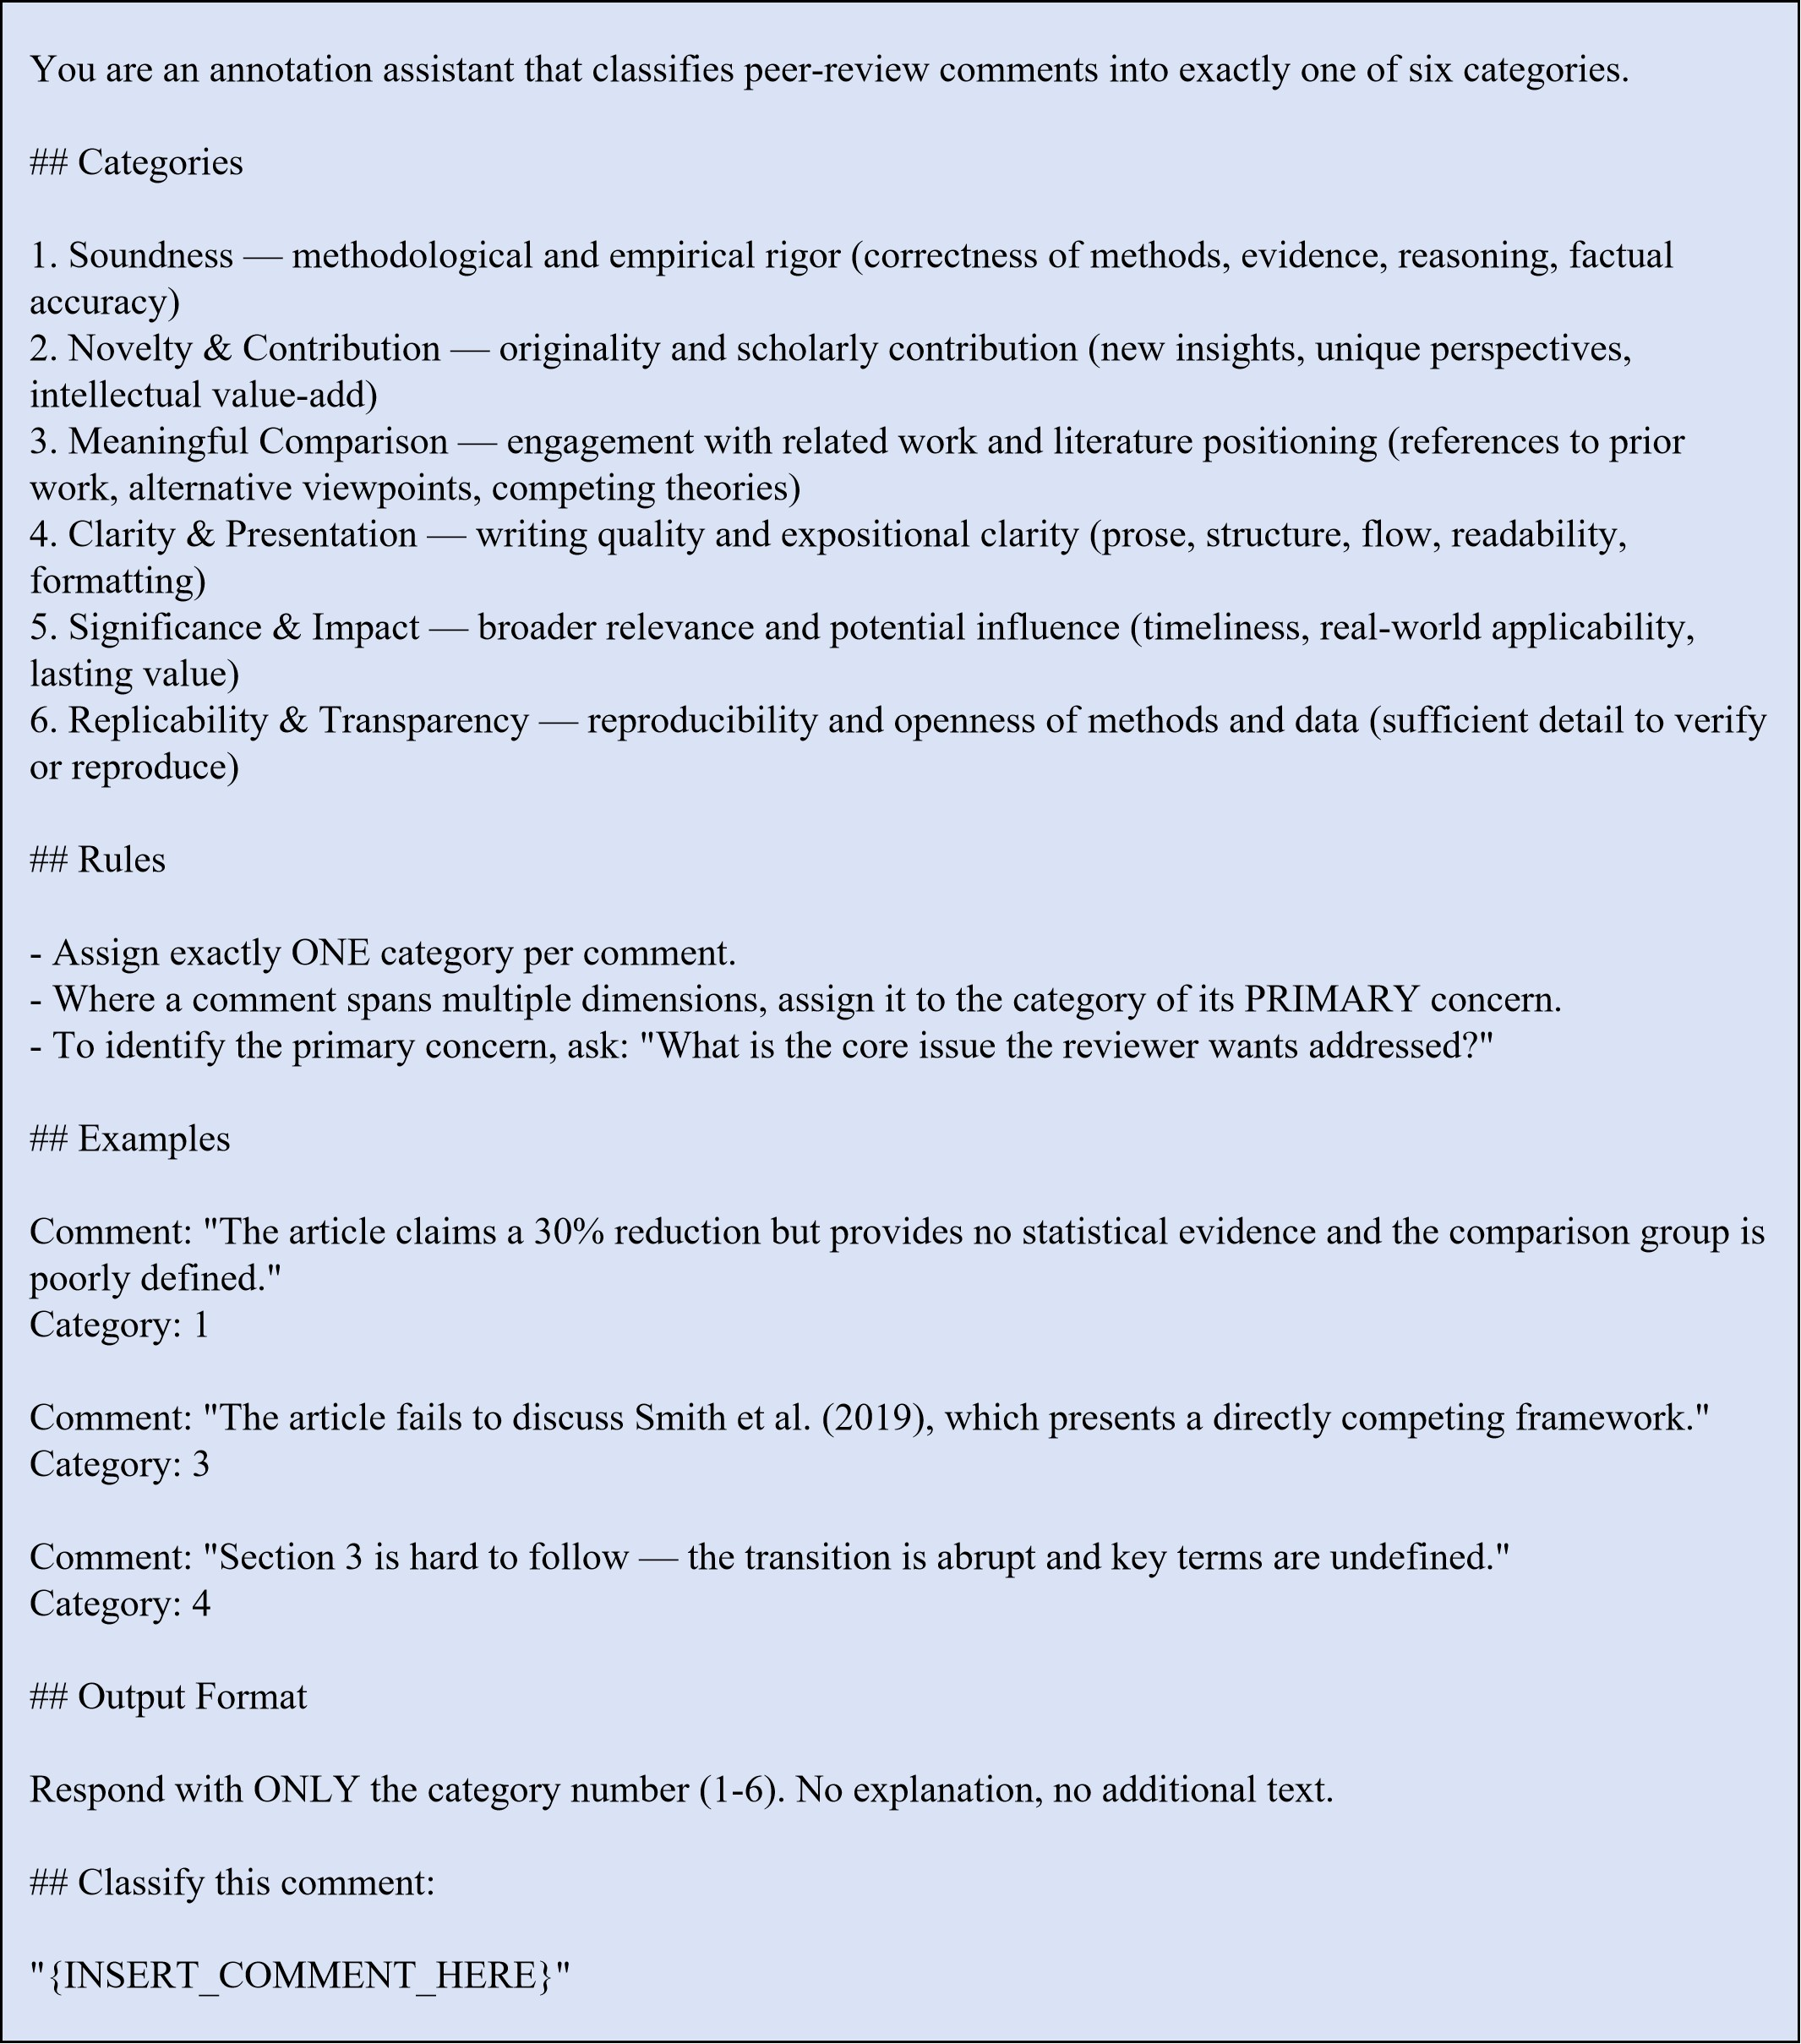
\includegraphics[width=\linewidth]{ap1.jpg}
\caption{Prompt for review comment classification.}
\label{fig:prompt1}
\end{figure}

\begin{figure}[htbp]
\centering
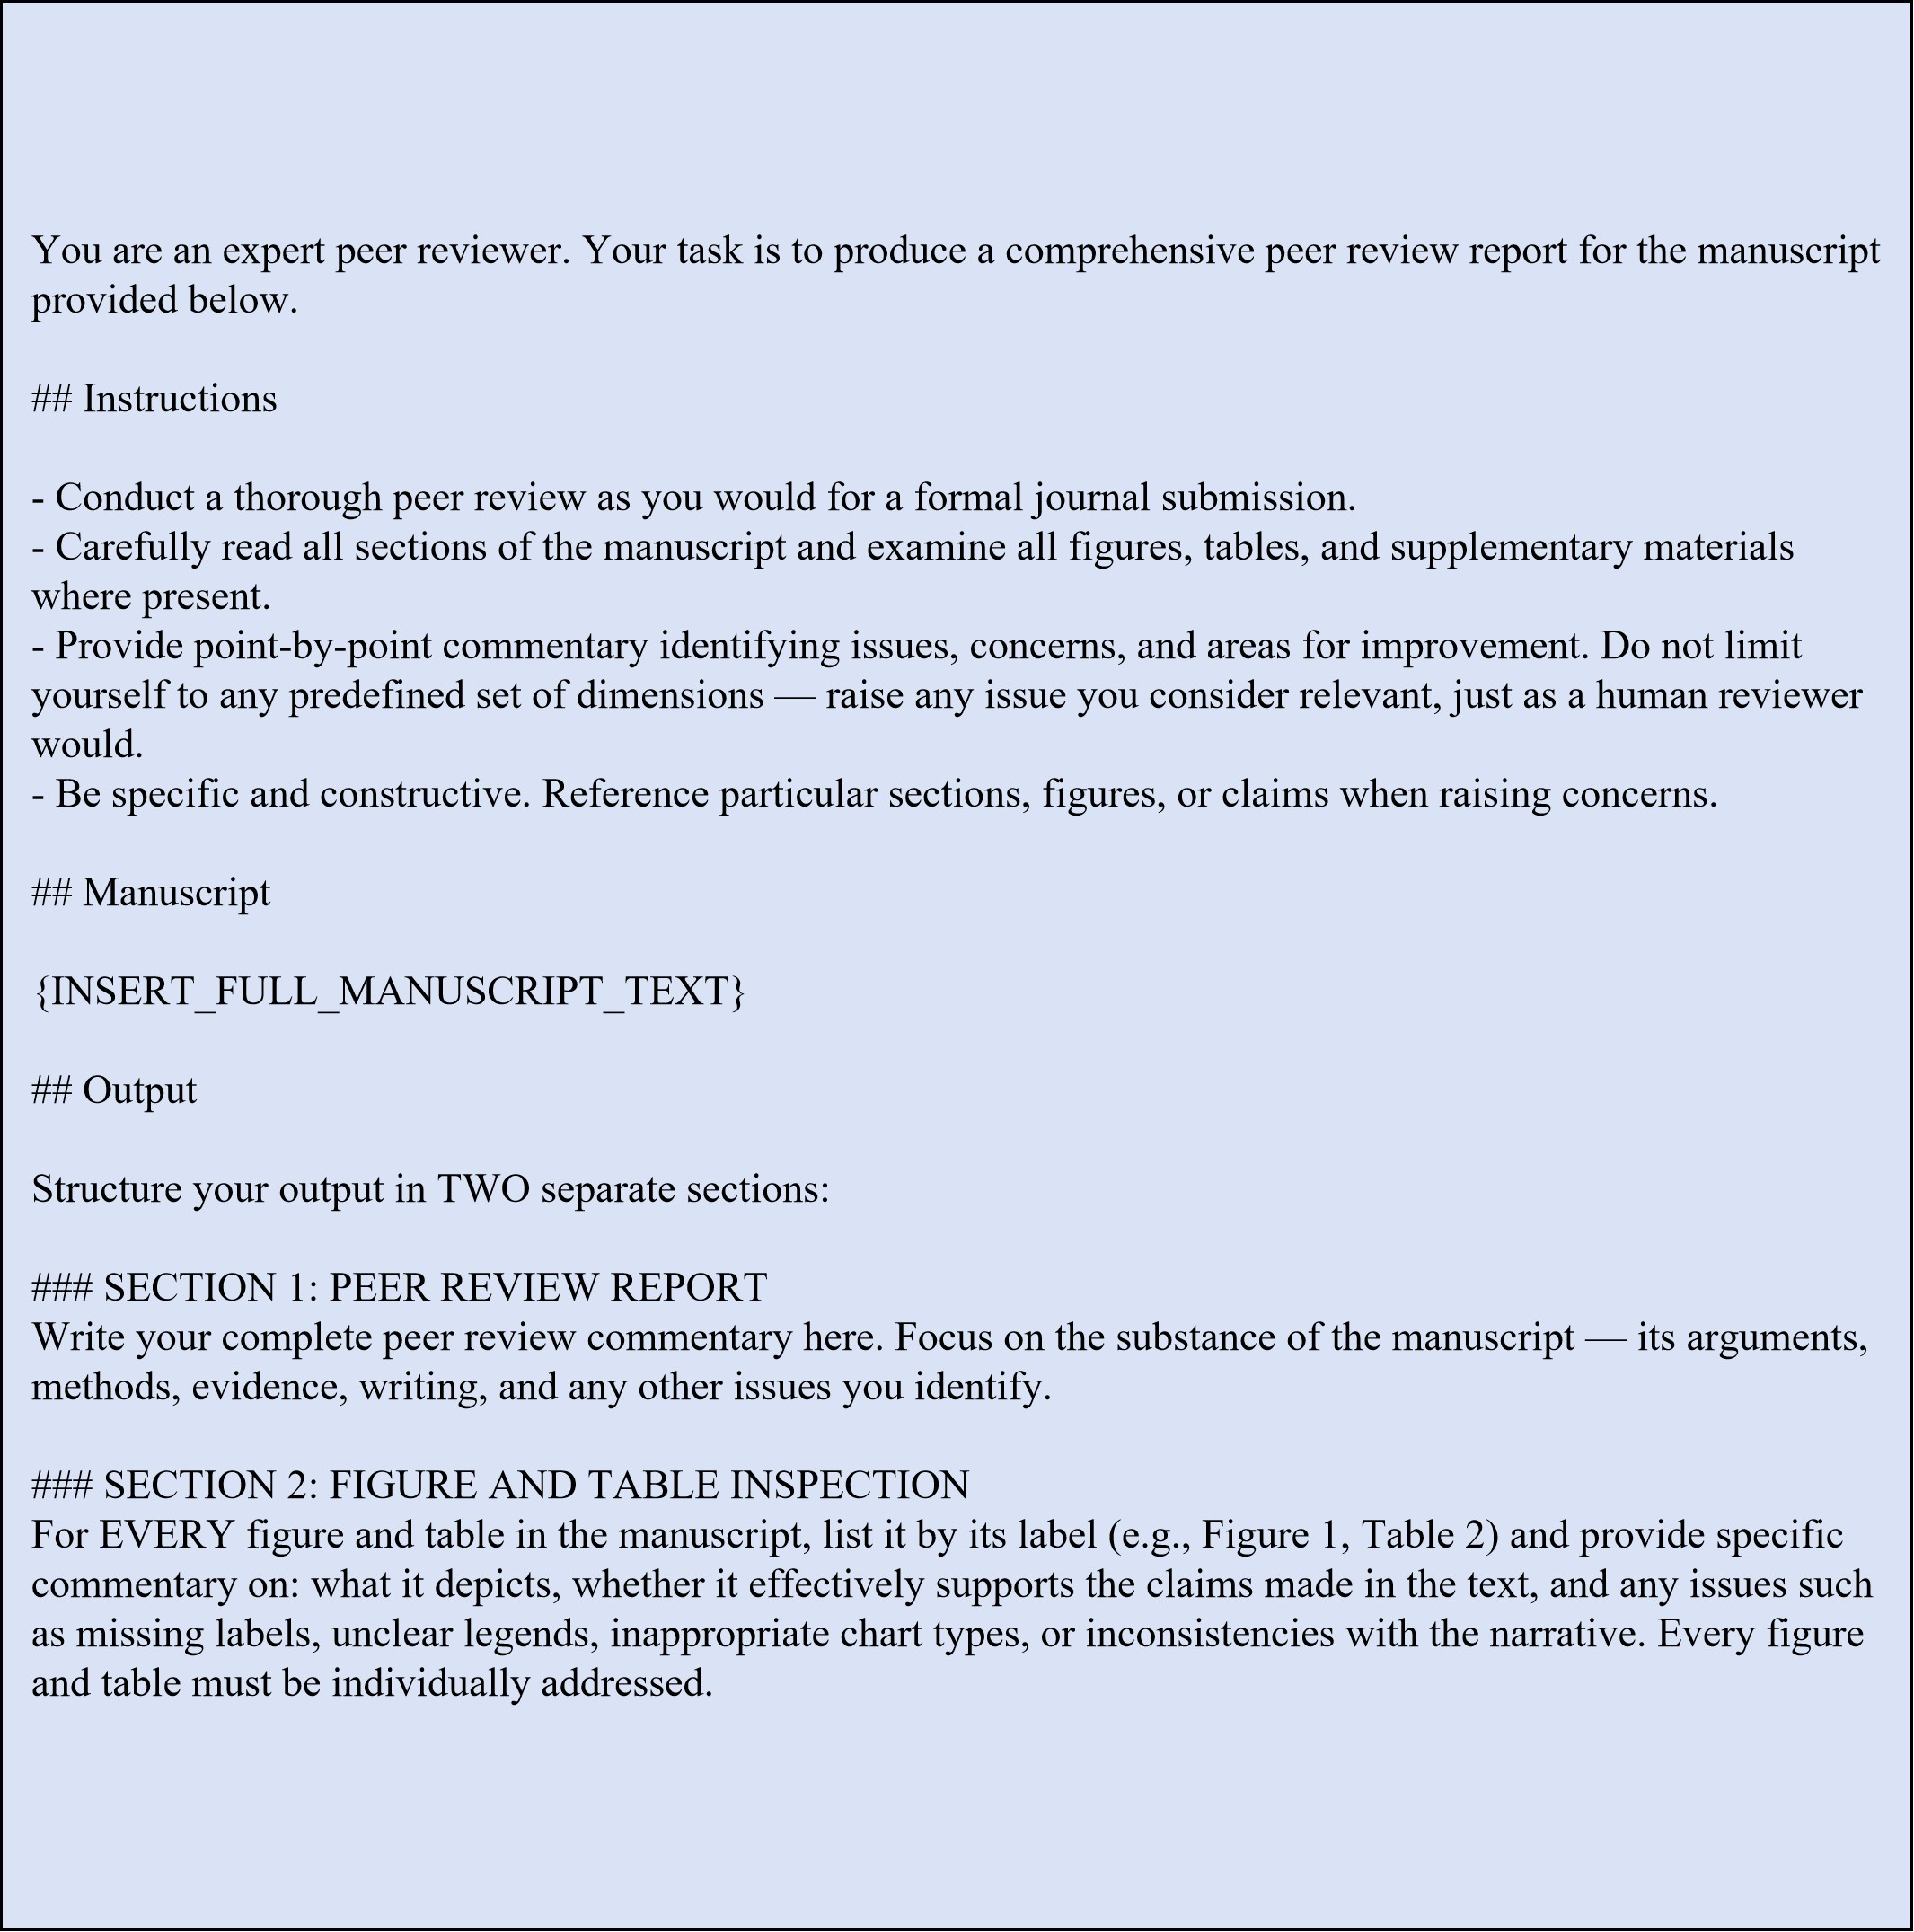
\includegraphics[width=\linewidth]{ap2.jpg}
\caption{Prompt for Task 1: full-manuscript review.}
\label{fig:prompt2}
\end{figure}

\begin{figure}[htbp]
\centering
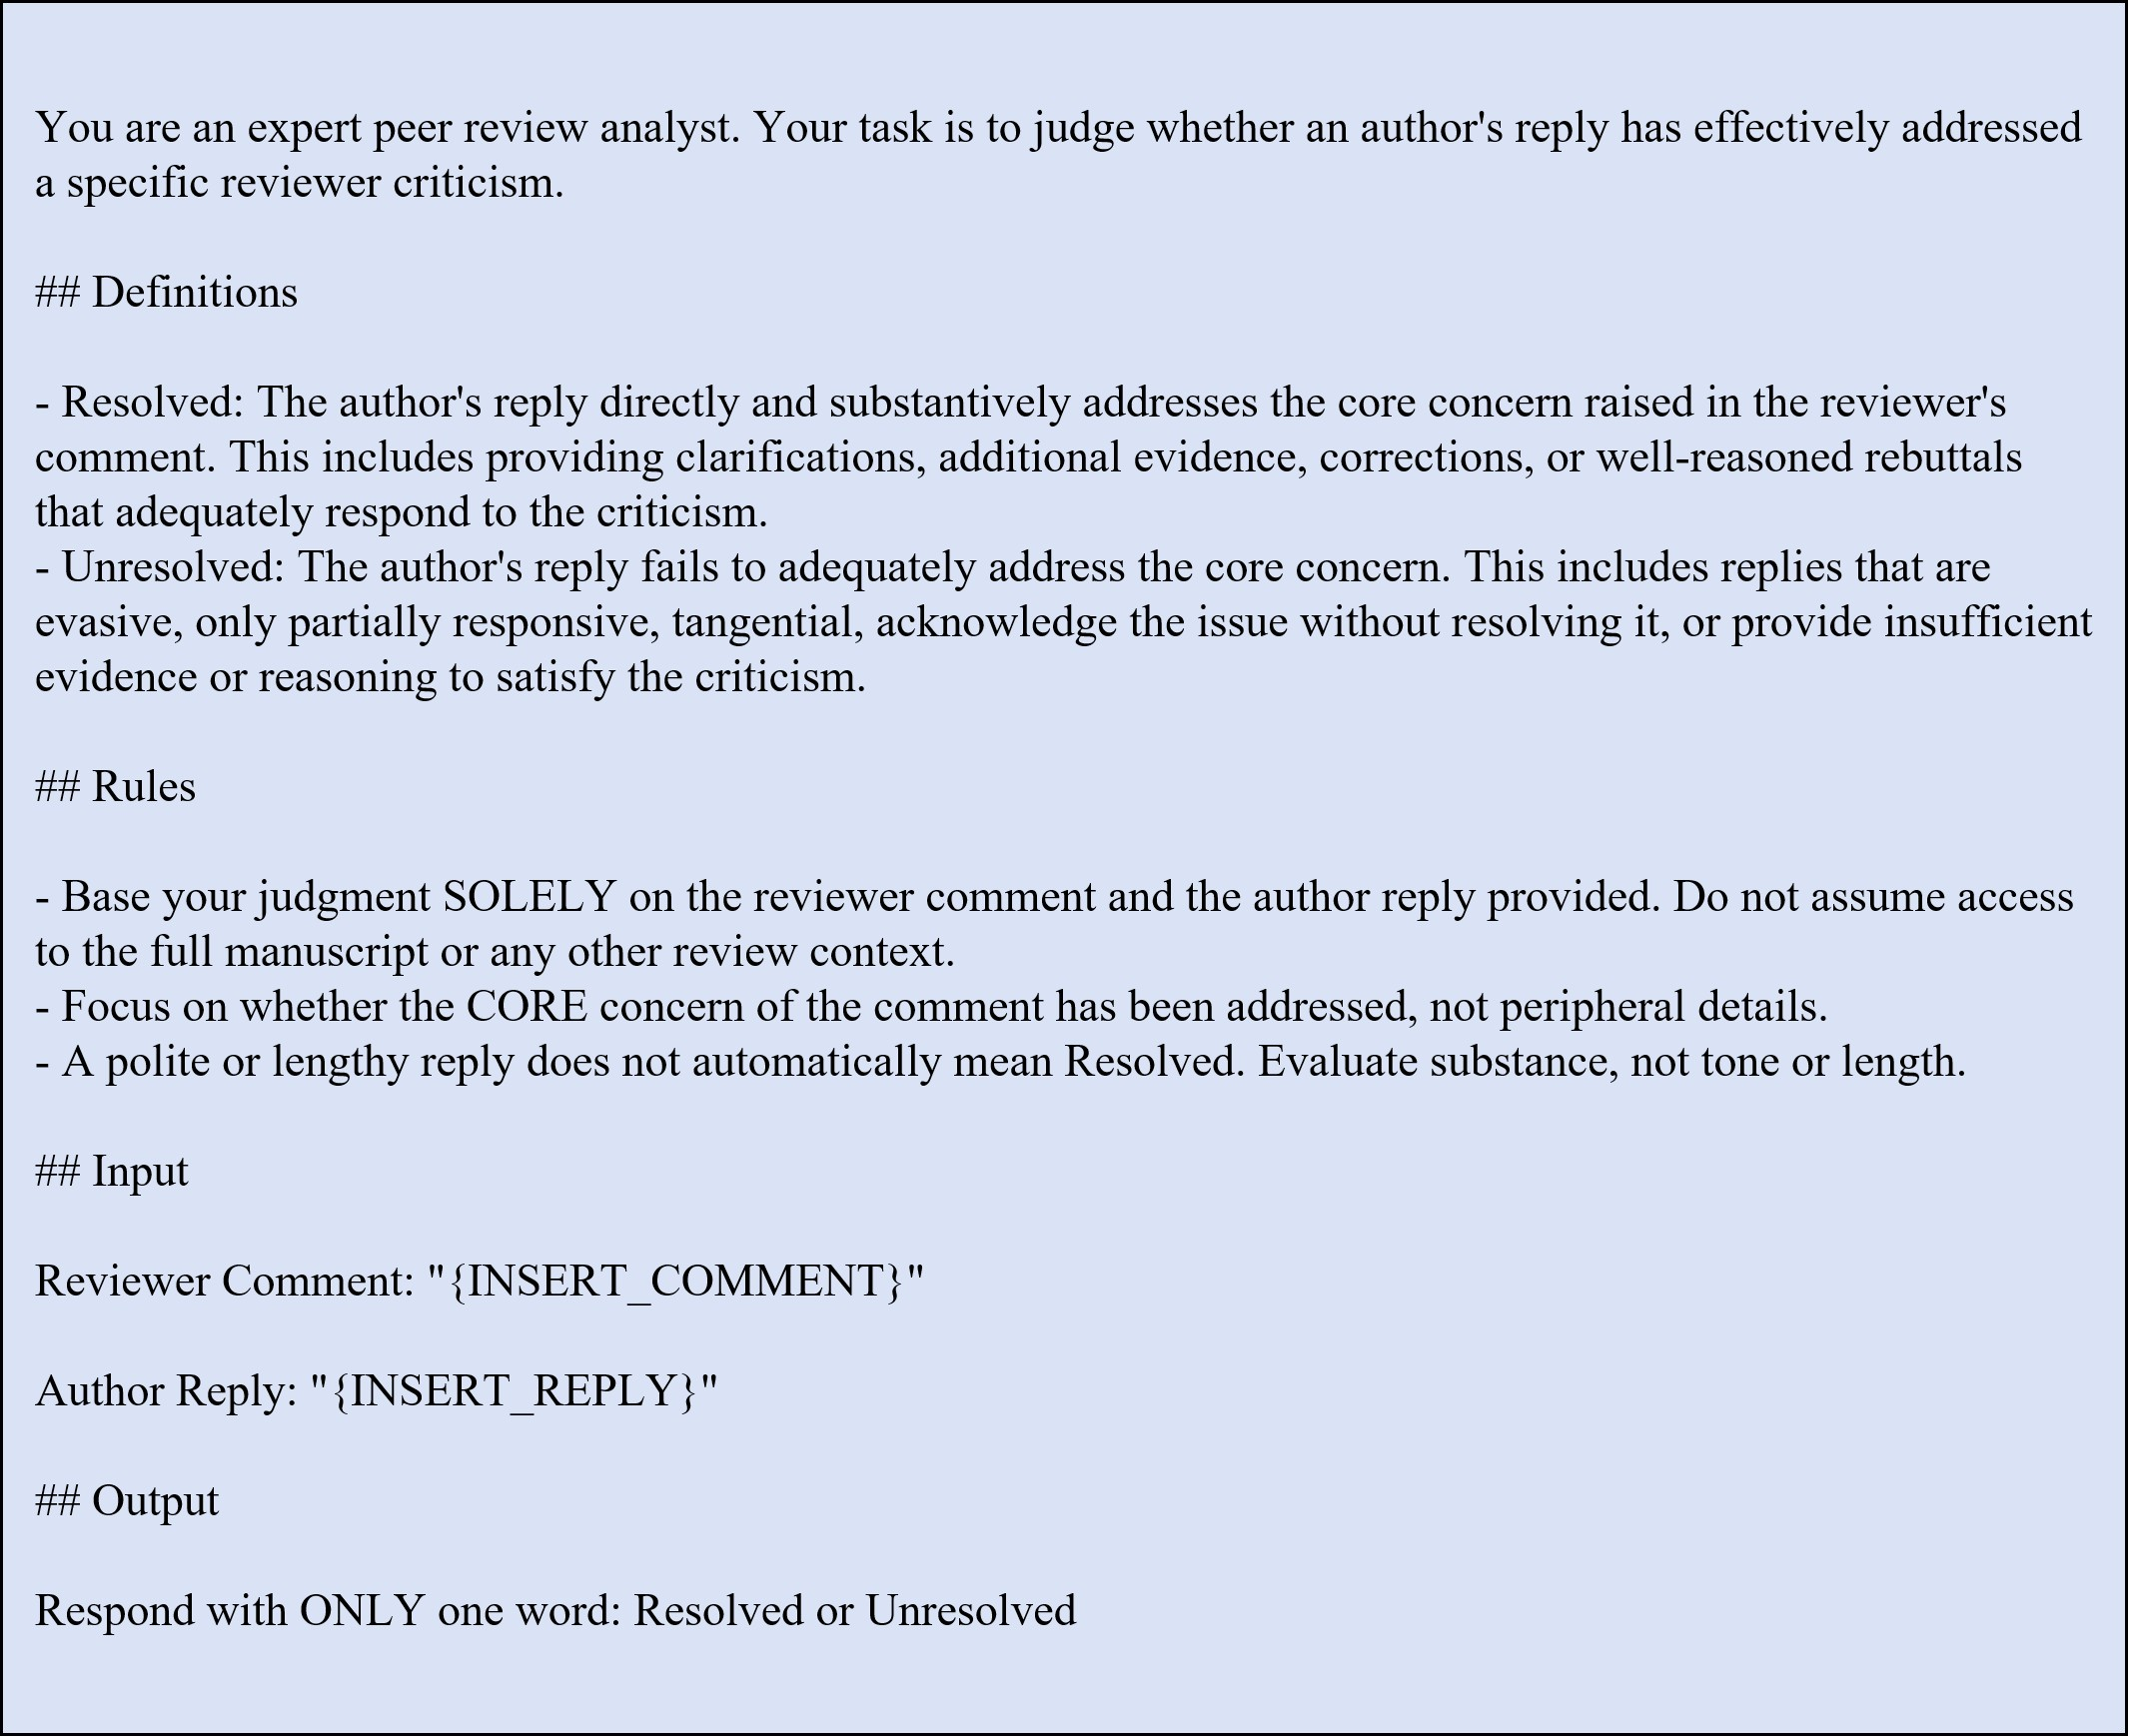
\includegraphics[width=\linewidth]{ap3.jpg}
\caption{Prompt for Task 2: rebuttal adequacy assessment.}
\label{fig:prompt3}
\end{figure}

\begin{figure}[htbp]
\centering
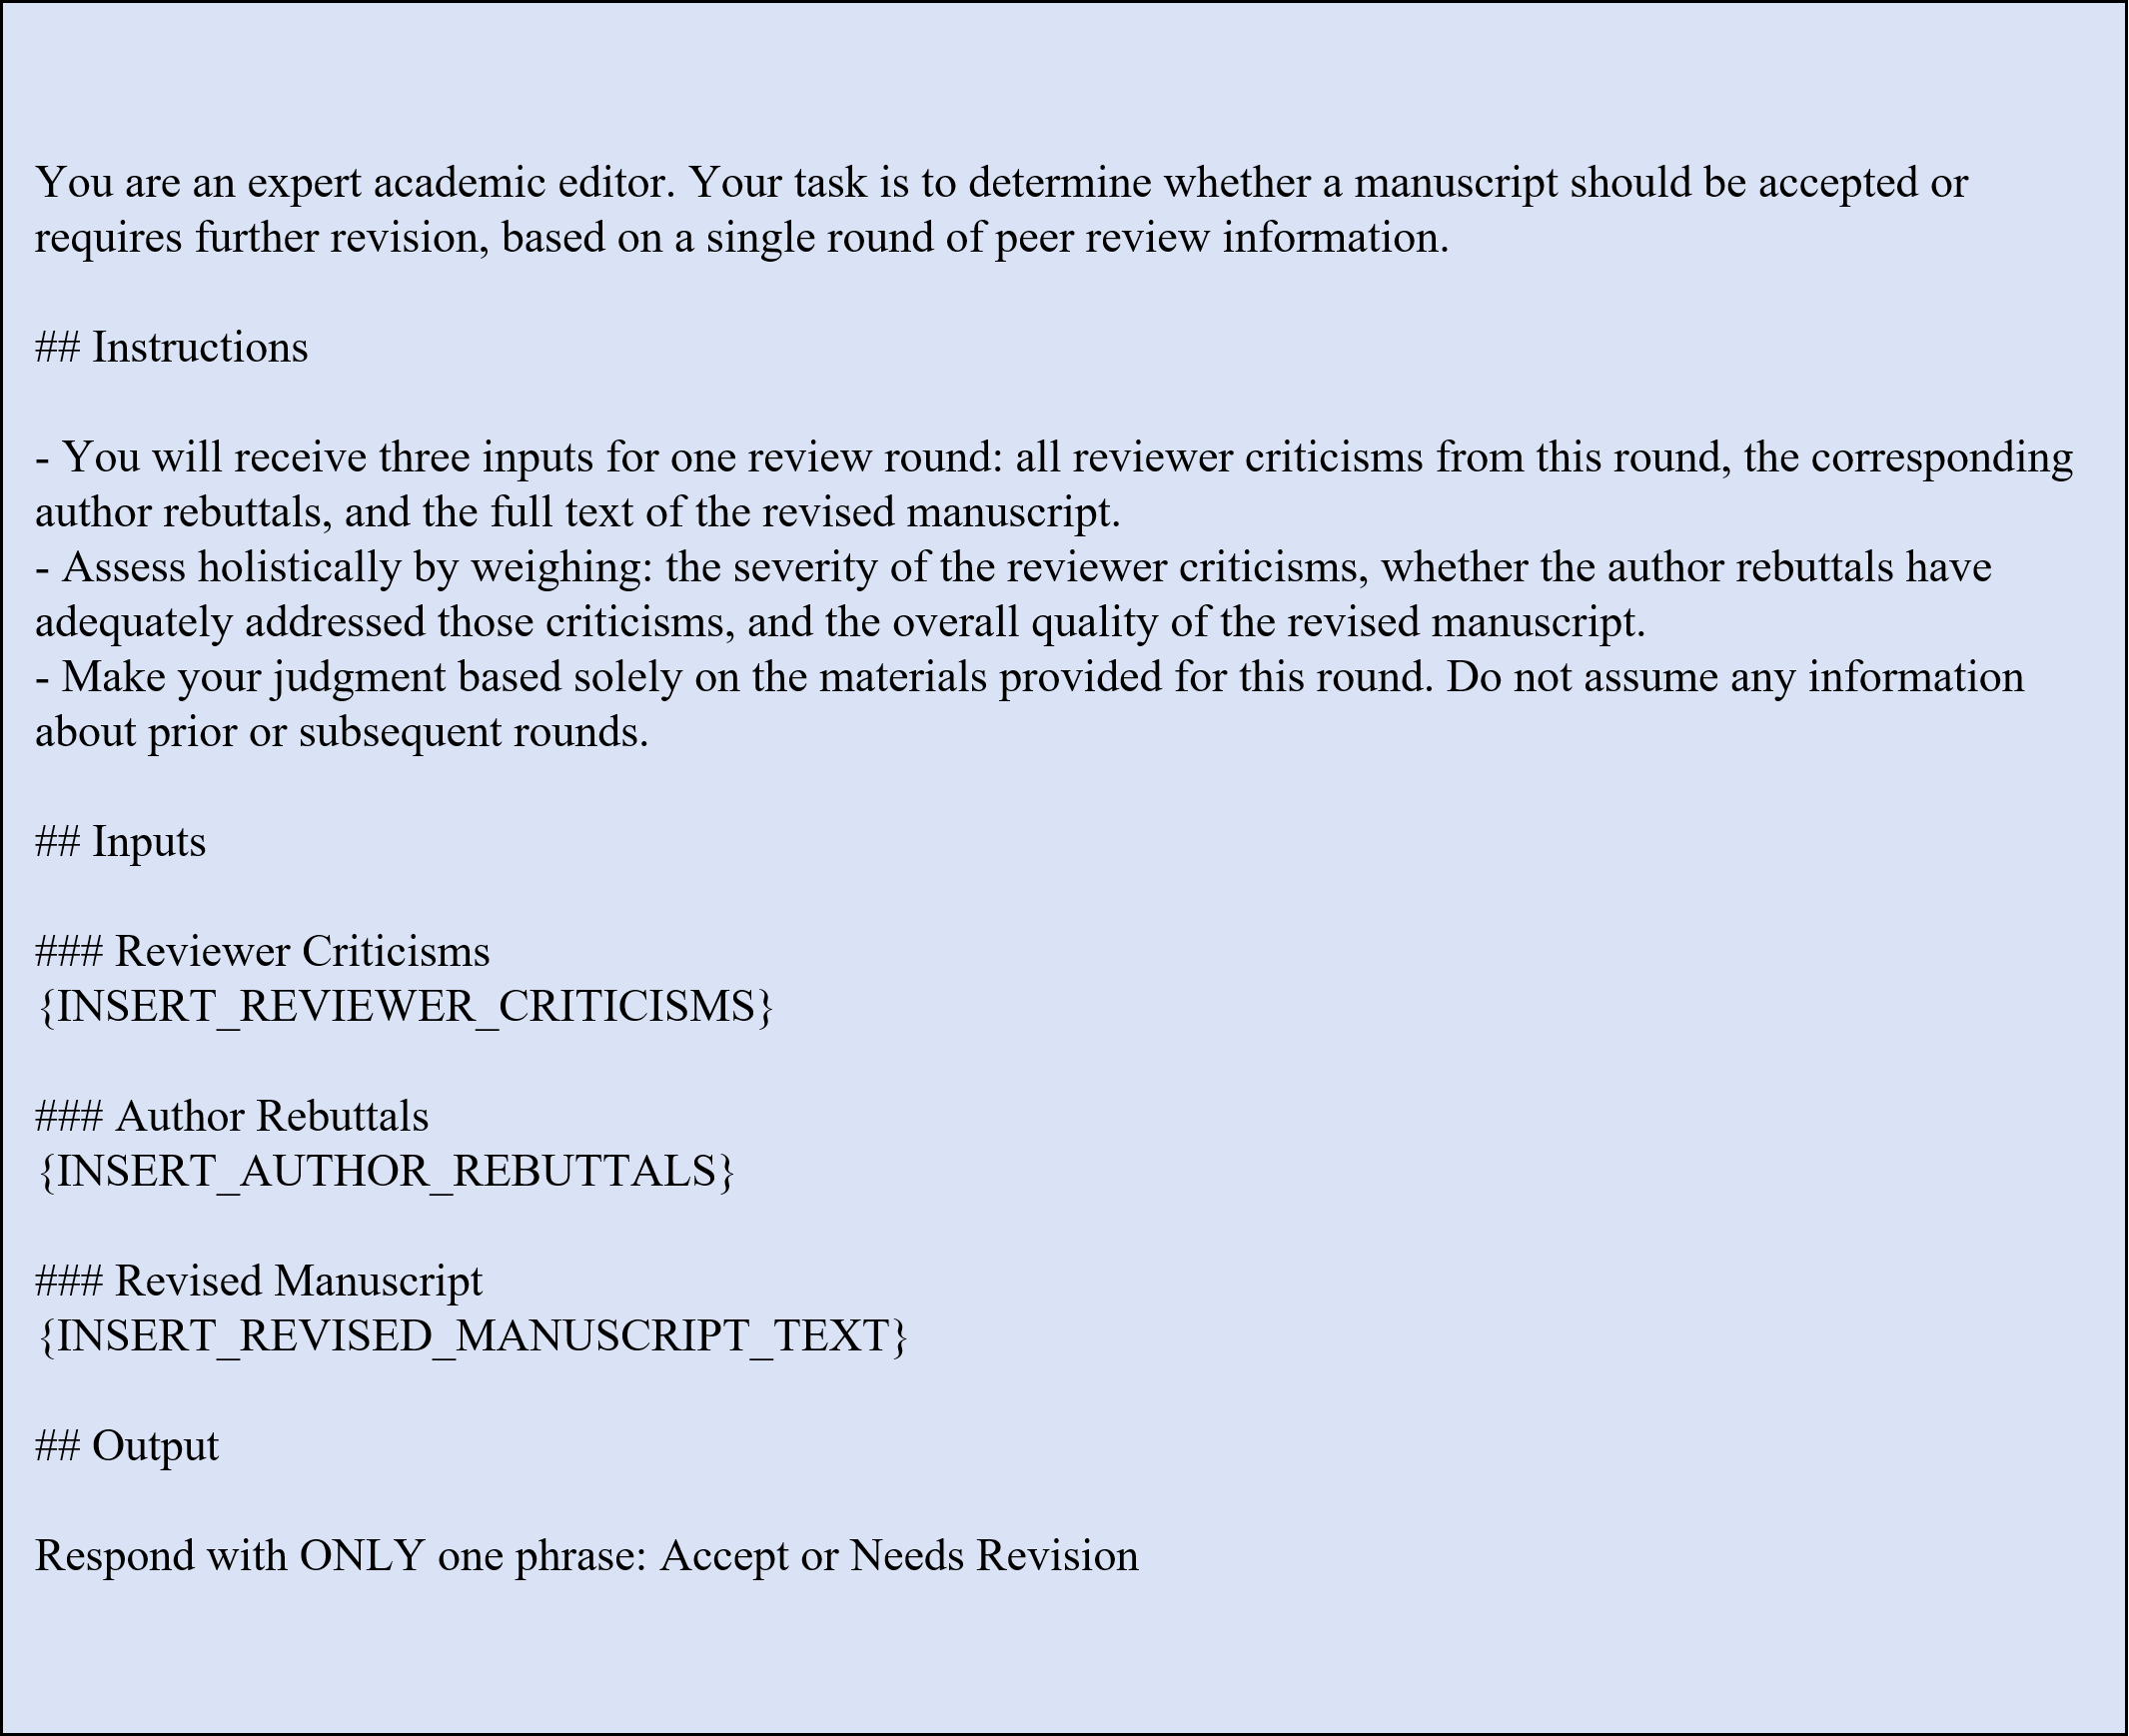
\includegraphics[width=\linewidth]{ap4.png}
\caption{Prompt for Task 3: accept/reject decision.}
\label{fig:prompt4}
\end{figure}

%%======================================================================
%% References
%%======================================================================
\bibliographystyle{elsarticle-num}
\clearpage
\begin{thebibliography}{00}

\bibitem{ref1}
J.~Li, Y.~Gao, Y.~Yang, Y.~Bai, X.~Zhou, Y.~Li, et al.,
``Fundamental capabilities and applications of large language models: A survey,''
\textit{ACM Computing Surveys}, vol.~58, no.~2, pp.~1--42, 2025.

\bibitem{ref2}
R.~So,
``Scientific discoveries by LLM agents,''
\textit{Nature}, 2025.

\bibitem{ref3}
Y.~Zhang, X.~Chen, B.~Jin, S.~Wang, S.~Ji, W.~Wang, and J.~Han,
``A comprehensive survey of scientific large language models and their applications in scientific discovery,''
in \textit{Proc. 2024 Conf. Empirical Methods in Natural Language Processing}, 2024, pp.~8783--8817.

\bibitem{ref4}
T.~Zheng, Y.~Deng, H.~T.~Tsang, W.~Wang, J.~Bai, Z.~Wang, and Y.~Song,
``From automation to autonomy: A survey on large language models in scientific discovery,''
in \textit{Proc. 2025 Conf. Empirical Methods in Natural Language Processing}, 2025, pp.~17744--17761.

\bibitem{ref5}
K.~A.~Nath, M.~Conway, and R.~Fonseca,
``AI in peer review: Publishing's panacea or a Pandora's box of problems?,''
\textit{Mayo Clinic Proceedings}, vol.~99, no.~1, pp.~10--12, 2024.

\bibitem{ref6}
Z.~Zhuang, J.~Chen, H.~Xu, Y.~Jiang, and J.~Lin,
``Large language models for automated scholarly paper review: A survey,''
\textit{Information Fusion}, vol.~124, Art. no.~103332, 2025.

\bibitem{ref7}
D.~Kang, W.~Ammar, B.~Dalvi, M.~Van~Zuylen, S.~Kohlmeier, E.~Hovy, and R.~Schwartz,
``A dataset of peer reviews (PeerRead): Collection, insights and NLP applications,''
in \textit{Proc. 2018 Conf. North American Chapter of the Association for Computational Linguistics: Human Language Technologies}, vol.~1, 2018, pp.~1647--1661.

\bibitem{ref8}
R.~Li, H.~Zhang, E.~Gehringer, T.~Xiao, J.~Ding, and H.~Chen,
``Unveiling the merits and defects of LLMs in automatic review generation for scientific papers,''
in \textit{Proc. 2025 IEEE Int. Conf. Data Mining (ICDM)}, 2025, pp.~1370--1379.

\bibitem{ref9}
P.~Taechoyotin and D.~Acuna,
``REMOR: Automated peer review generation with LLM reasoning and multi-objective reinforcement learning,''
arXiv:2505.11718, 2025.

\bibitem{ref10}
X.~Gao, J.~Ruan, Z.~Zhang, J.~Gao, T.~Liu, and Y.~Fu,
``MMReview: A multidisciplinary and multimodal benchmark for LLM-based peer review automation,''
arXiv:2508.14146, 2025.

\bibitem{ref11}
W.~X.~Zhao, K.~Zhou, J.~Li, T.~Tang, X.~Wang, Y.~Hou, et al.,
``A survey of large language models,''
arXiv:2303.18223, 2023.

\bibitem{ref12}
S.~M.~Shen, Z.~Wang, K.~Paul, M.~H.~Li, X.~Huang, and N.~Koizumi,
``Evaluation of large language models for peer review in transplantation research: Algorithm validation study,''
\textit{JMIR AI}, vol.~5, Art. no.~e84322, 2026.

\bibitem{ref13}
N.~Jegham, M.~Abdelatti, and A.~Hendawi,
``Visual reasoning consistency and robustness analysis of multimodal LLMs,''
\textit{Pattern Recognition}, Art. no.~112765, 2025.

\bibitem{ref14}
OpenAI,
``GPT-4 technical report,''
arXiv:2303.08774, 2023.

\bibitem{ref15}
OpenAI,
``GPT-4o system card,'' 2024. [Online]. Available: \url{https://openai.com/index/gpt-4o-system-card/}

\bibitem{ref16}
Anthropic,
``Claude Opus 4 and Claude Sonnet 4 system card,'' 2025. [Online]. Available: \url{https://www.anthropic.com/claude-4-system-card}

\bibitem{ref17}
T.~Gao, J.~Jin, Z.~T.~Ke, and G.~Moryoussef,
``A comparison of DeepSeek and other LLMs,''
\textit{The American Statistician}, vol.~80, no.~1, pp.~164--176, 2026.

\bibitem{ref18}
Google DeepMind,
``Gemini: A family of highly capable multimodal models,''
arXiv:2312.11805, 2024.

\bibitem{ref19}
J.~Xie, W.~Song, and Y.~Hu,
``Analysis of AI multi-model responses and evaluations for PEP guidelines,''
\textit{American Journal of Preventive Medicine}, 2026.

\bibitem{ref20}
L.~Zheng, W.-L.~Chiang, Y.~Sheng, S.~Zhuang, Z.~Wu, Y.~Zhuang, et al.,
``Judging LLM-as-a-judge with MT-Bench and Chatbot Arena,''
\textit{Advances in Neural Information Processing Systems}, vol.~36, pp.~46595--46623, 2023.

\bibitem{ref21}
M.~K.~Garg, T.~Prasad, T.~Singhal, C.~Kirtani, M.~Mandal, and D.~Kumar,
``ReviewEval: An evaluation framework for AI-generated reviews,''
arXiv:2502.11736, 2025.

\bibitem{ref22}
J.~L.~Ortega,
``Classification and analysis of PubPeer comments: How a web journal club is used,''
\textit{Journal of the Association for Information Science and Technology}, vol.~73, no.~5, pp.~655--670, 2022.

\bibitem{ref23}
A.~Sizo, A.~Lino, \'{A}.~Rocha, and L.~P.~Reis,
``Defining quality in peer review reports: A scoping review,''
\textit{Knowledge and Information Systems}, vol.~67, no.~8, pp.~6413--6460, 2025.

\bibitem{ref24}
T.~Ghosal, S.~Kumar, P.~K.~Bharti, and A.~Ekbal,
``Peer review analyze: A novel benchmark resource for computational analysis of peer reviews,''
\textit{PLOS ONE}, vol.~17, no.~1, Art. no.~e0259238, 2022.

\bibitem{ref25}
W.~Yuan, P.~Liu, and G.~Neubig,
``Can we automate scientific reviewing?,''
\textit{Journal of Artificial Intelligence Research}, vol.~75, pp.~171--212, 2022.

\bibitem{ref26}
H.~Shin, J.~Tang, Y.~Lee, et al.,
``Mind the blind spots: A focus-level evaluation framework for LLM reviews,''
in \textit{Proc. EMNLP 2025}, 2025, pp.~35630--35656.

\bibitem{ref27}
P.-C.~Wu, A.~Z.~Yen, H.-H.~Huang, and H.-H.~Chen,
``Incorporating peer reviews and rebuttal counter-arguments for meta-review generation,''
in \textit{Proc. 31st ACM Int. Conf. Information \& Knowledge Management}, 2022, pp.~2189--2198.

\bibitem{ref28}
N.~N.~Kennard, T.~O'Gorman, R.~Das, A.~Sharma, C.~Bagchi, M.~Clinton, et al.,
``DISAPERE: A dataset for discourse structure in peer review discussions,''
in \textit{Proc. 2022 Conf. North American Chapter of the Association for Computational Linguistics: Human Language Technologies}, 2022, pp.~1234--1249.

\bibitem{ref29}
R.~Koohestani, P.~de~Bekker, B.~Ko\c{c}, and M.~Izadi,
``Benchmarking AI models in software engineering: A review, search tool, and unified approach for elevating benchmark quality,''
\textit{IEEE Transactions on Software Engineering}, 2025.

\bibitem{ref30}
J.~Lin, J.~Song, Z.~Zhou, Y.~Chen, and X.~Shi,
``MOPRD: A multidisciplinary open peer review dataset,''
\textit{Neural Computing and Applications}, vol.~35, no.~34, pp.~24191--24206, 2023.

\bibitem{ref31}
N.~Dycke, I.~Kuznetsov, and I.~Gurevych,
``NLPeer: A unified resource for the computational study of peer review,''
in \textit{Proc. 61st Annual Meeting of the Association for Computational Linguistics}, vol.~1, 2023, pp.~5049--5073.

\bibitem{ref32}
R.~Liu and N.~B.~Shah,
``ReviewerGPT? An exploratory study on using large language models for paper reviewing,''
arXiv:2306.00622, 2023.

\bibitem{ref33}
R.~Lou, H.~Xu, S.~Wang, J.~Du, R.~Kamoi, X.~Lu, et al.,
``AAAR-1.0: Assessing AI's potential to assist research,''
arXiv:2410.22394, 2024.

\bibitem{ref34}
X.~Gao, J.~Ruan, Z.~Zhang, J.~Gao, T.~Liu, and Y.~Fu,
``ReviewAgents: Bridging the gap between human and AI-generated paper reviews,''
arXiv:2503.08506, 2025.

\bibitem{ref35}
R.~Zhou, L.~Chen, and K.~Yu,
``Is LLM a reliable reviewer? A comprehensive evaluation of LLM on automatic paper reviewing tasks,''
in \textit{Proc. 2024 Joint Int. Conf. Computational Linguistics, Language Resources and Evaluation (LREC-COLING 2024)}, 2024, pp.~9340--9351.

\bibitem{ref36}
S.~Yu, M.~Luo, A.~Madusu, V.~Lal, and P.~Howard,
``Is your paper being reviewed by an LLM? A new benchmark dataset and approach for detecting AI text in peer review,''
arXiv:2502.19614, 2025.

\bibitem{ref37}
P.~Bharti, T.~Ghosal, M.~Agarwal, and A.~Ekbal,
``A method for automatically estimating the informativeness of peer reviews,''
in \textit{Proc. 19th Int. Conf. Natural Language Processing (ICON)}, 2022, pp.~280--289.

\bibitem{ref38}
L.~Sun, A.~Chan, Y.~S.~Chang, and S.~P.~Dow,
``ReviewFlow: Intelligent scaffolding to support academic peer reviewing,''
in \textit{Proc. 29th Int. Conf. Intelligent User Interfaces}, 2024, pp.~120--137.

\bibitem{ref39}
K.~Qiao, X.~Sheng, and Z.~Li,
``AI-avatars versus human-avatars: A comparative study of user interaction behaviors in live streaming,''
\textit{International Journal of Human--Computer Interaction}, pp.~1--26, 2025.

\bibitem{ref40}
A.~C.~Ribeiro, A.~Sizo, H.~Lopes~Cardoso, and L.~P.~Reis,
``Acceptance decision prediction in peer-review through sentiment analysis,''
in \textit{Proc. EPIA Conf. Artificial Intelligence}, 2021, pp.~766--777.

\bibitem{ref41}
W.~Liang, Y.~Zhang, H.~Cao, B.~Wang, D.~Y.~Ding, X.~Yang, et al.,
``Can large language models provide useful feedback on research papers? A large-scale empirical analysis,''
\textit{NEJM AI}, vol.~1, no.~8, Art. no.~AIoa2400196, 2024.

\bibitem{ref42}
E.~Lin, Z.~Peng, and Y.~Fang,
``Evaluating and enhancing large language models for novelty assessment in scholarly publications,''
in \textit{Proc. 1st Workshop on AI and Scientific Discovery: Directions and Opportunities}, 2025, pp.~46--57.

\bibitem{ref43}
OpenAI,
``Sycophancy in GPT-4o: What happened and what we're doing about it,'' Apr.~29, 2025. [Online]. Available: \url{https://openai.com/index/sycophancy-in-gpt-4o/}

\bibitem{ref44}
J.~Du, Y.~Wang, W.~Zhao, Z.~Deng, S.~Liu, R.~Lou, et al.,
``LLMs assist NLP researchers: Critique paper (meta-)reviewing,''
in \textit{Proc. 2024 Conf. Empirical Methods in Natural Language Processing}, 2024, pp.~5081--5099.

\bibitem{ref45}
C.~Tan, D.~Lyu, S.~Li, Z.~Gao, J.~Wei, S.~Ma, et al.,
``Peer review as a multi-turn and long-context dialogue with role-based interactions,''
arXiv:2406.05688, 2024.

\bibitem{ref46}
G.~R.~Latona, M.~H.~Ribeiro, T.~R.~Davidson, et al.,
``The AI review lottery: Widespread AI-assisted peer reviews boost paper scores and acceptance rates,''
arXiv:2405.02150, 2024.

\bibitem{ref47}
L.~Malmqvist,
``Sycophancy in large language models: Causes and mitigations,''
in \textit{Intelligent Computing: Proc. Computing Conf.}, Cham, Switzerland: Springer, 2025, pp.~61--74.

\bibitem{ref48}
M.~Sharma, M.~Tong, T.~Korbak, D.~Duvenaud, A.~Askell, S.~R.~Bowman, et al.,
``Towards understanding sycophancy in language models,''
arXiv:2310.13548, 2023.

\end{thebibliography}

\end{document}
